\documentclass[fontset=windows]{article}
\usepackage[margin=1in]{geometry}%设置边距,符合Word设定
\usepackage{ctex}
\usepackage{setspace}
\usepackage{lipsum}
\usepackage{graphicx}%插入图片
\usepackage{listings}
\usepackage[dvipsnames]{xcolor}
\usepackage[centerlast]{caption}
\usepackage{pifont}
\graphicspath{{Figures/}}%文章所用图片在当前目录下的 Figures目录
\usepackage{hyperref} % 对目录生成链接,注:该宏包可能与其他宏包冲突,故放在所有引用的宏包之后


\usepackage{xcolor}
\usepackage{listings}
\definecolor{codeblue}{RGB}{0, 0, 255}
\definecolor{codegreen}{RGB}{0, 128, 0}
\definecolor{codegray}{RGB}{128, 128, 128}
\definecolor{codepurple}{RGB}{128, 0, 128}
\definecolor{codeorange}{RGB}{255, 165, 0}
\definecolor{backcolour}{RGB}{255, 255, 255}
\definecolor{Lightskyblue}{RGB}{61, 176, 247}
\definecolor{classcolour}{RGB}{21, 178, 129}
\definecolor{codeyellow}{RGB}{255, 207, 64}
\definecolor{lightpurple}{RGB}{225, 105, 204}




\makeatletter
\renewcommand{\@seccntformat}[1]{\csname the#1\endcsname\quad}
\makeatother

\lstdefinestyle{cppstyle}
{
    language=C++,
	sensitive=true,
	basicstyle=\ttfamily\small,
    keywordstyle=\bfseries\color{codeblue}, %关键词高亮
    commentstyle=\itshape\color{codegreen}, %注释高亮
    stringstyle=\color{codeorange}, %字符串高亮
    identifierstyle=\color{black},
    numbers=left,
    numberstyle=\tiny\color{codegray},
    stepnumber=1,
    numbersep=5pt,
    backgroundcolor=\color{backcolour},
    showspaces=false,
    showstringspaces=false,
    showtabs=false,
    frame=single,
    rulecolor=\color{black},
    tabsize=4,
    captionpos=b, % 将标题位置设置为底部
    breaklines=true, %自动换行
    breakatwhitespace=false, %无需括号的自动换行
    title=\lstname,
    escapeinside={\%*}{*},
    morekeywords={constexpr, nullptr, bool, true, false},
	morekeywords = [2]{count00,flag,record1,record2,count,GPA,ID,lecture,name,rank,score,term,type,err,next,safe,warning,a,b,head,slice,ave_GPA,count,number,total_score,GPA_related_score,GPA_term,score_term,total_GPA,total_GPA_term},
	keywordstyle=[2]\color{Lightskyblue},
	moreemph = [3]{while,for,if,else,elseif},
	emphstyle=[3]\color{codepurple},
    moreemph = [1]{Node,people,LinkedList,basic,student,course,HANDLE},
	emphstyle=[1]\color{classcolour},
	moreemph = [2]{strcat,strcmp,strcpy,check,input,input_choice,input_GPA,wrong,SetConsoleTextAttribute,endl,clear,good,ignore,typewrong,input_score,input_term,input_ID,check,input,typewrong,addNode,pickoutNode,output,welcome,case1,case2,case3,case4,case5,finish,pipei,shuru,prepare,main},
	emphstyle=[2]\color{codeyellow},
	moreemph = [4]{STD_OUTPUT_HANDLE,FOREGROUND_RED,FOREGROUND_INTENSITY,FOREGROUND_GREEN,FOREGROUND_BLUE,NULL},
	emphstyle=[4]\color{lightpurple},
}


\hypersetup{colorlinks = true,  % 将链接文字带颜色
	bookmarksopen = true, % 展开书签
	bookmarksnumbered = true, % 书签带章节编号
	pdftitle = This is a testfile for vscode, % 标题
	pdfauthor =Ali-loner} % 作者
\bibliographystyle{plain}% 参考文献引用格式

\newcommand{\upcite}[1]{\textsuperscript{\cite{#1}}}
\renewcommand{\thesection}{\arabic{section}}
\renewcommand{\contentsname}{\centerline{\heiti\zihao{3}目\hspace{2cm}录}} %经过设置word格式后,将目录标题居中
%*********************封面页*********************

\title{\heiti\zihao{0}程{ }序{ }设{ }计{ }报{ }告}
\author{}
\date{}

\begin{document}
\maketitle
\begin{center}
\songti\zihao{3}课程名称\underline{{ }{ }{ }计算机程序设计基础2{ }{ }{ }}
\\
\vspace{8cm}   
\songti\zihao{3}班\hspace{1.128cm}级\underline{\hspace{2.7cm}无28\hspace{2.7cm}}
\\
\songti\zihao{3}学\hspace{1.128cm}号\underline{\hspace{1.87cm}2022010722\hspace{1.87cm}}
\\
\songti\zihao{3}姓\hspace{1.128cm}名\underline{\hspace{2.4cm}赵子恒\hspace{2.4cm}}
\\
\vspace{3cm}
\date{\today}
\vfill
\newpage
\end{center}


%*********************目录*********************

%\begin{abstract}
%	\lipsum[2]
%\end{abstract}

\tableofcontents
\newpage
%*********************要求添加区域*******************
\section{设计内容与设计要求}
\subsection{课程设计目的}
面向对象程序设计课程设计是集中实践性环节之一,是学习完《计算机程序设计基础2》C++面向对象程序设计课程后进行的一次
全面的综合练习。要求学生达到熟练掌握C++语言的基本知识和技能;基本掌握面向对象程序设计的思想和方法;能够利用所学
的基本知识和技能,解决简单的面向对象程序设计问题,从而提高动手编程解决实际问题的能力。尤其重视创新思维培养。
\subsection{课题题目}
学生成绩管理系统(或公司人事管理系统)
\subsection{文档设计要求}

3.1 设计课题题目:每个同学都单独完成1道课题。后面有范题,仅供同学们参考,不列入本次课程设计的课题。

3.2 对于程设题目,按照范题的格式。自行虚构软件需求。并按照第4点要求,编写设计文档。基本要求系统中设计的类的数目不少于
4个,每个类中要有各自的属性(多于3个)和方法(多于3个);需要定义一个抽象类,采用继承方式派生这些类。并设计一个多
重继承的派生类。在程序设计中,引入虚函数的多态性、运算符重载等机制。

\subsection{程序设计的基本要求}
(1)要求利用面向对象的方法以及C++的编程思想来完成系统的设计;

(2)要求在设计的过程中,建立清晰的类层次;

(3)根据课题完成以下主要工作:

\hspace{1cm}\ding{172}完成系统需求分析:包括系统设计目的与意义;系统功能需求(系统流程图);输入输出的

\hspace{1cm}要求。

\hspace{1cm}\ding{173}完成系统总体设计:包括系统功能分析;系统功能模块划分与设计(系统功能模块图)。

\hspace{1cm}\ding{174}完成系统详细设计:数据文件;类层次图;界面设计与各功能模块实现。

\hspace{1cm}\ding{175}系统调试:调试出现的主要问题,编译语法错误及修改,重点是运行逻辑问题修改和调整。

\hspace{1cm}\ding{176}使用说明书及编程体会:说明如何使用你编写的程序,详细列出每一步的操作步骤。

\hspace{1cm}\ding{177}键源程序(带注释)。

(4)自己设计测试数据,将测试数据存在文件中,通过文件进行数据读写来获得测试结果。

(5)按规定格式完成课程设计报告,并在网络学堂上按时提交。

(6)不得抄袭他人程序、课程设计报告,每个人应独立完成,在程序和设计报告中体现自己的个性设计。

%*********************正文*********************
\section{系统需求分析}
学生成绩管理系统中记录着学生的成绩情况,包括学生各门课程的等级,总体排名,绩点,各学期均绩等信息。同时,我们设计
的学生成绩管理系统应该考虑到实际使用中,学生存在重名,因此还包含学号作为学生身份的唯一标识。该成绩管理系统也同时
被老师和学生使用,因此并不能支持简单的查询,还要具有录入,修改和删除记录的功能。因此,系统的主要功能有以下六条:
\begin{enumerate}
	\item 录入学生成绩:作为成绩管理系统,录入学生成绩是必不可少的功能。该系统应该可以通过键盘,用学生的姓名和学
	号确定唯一的学生并将新的课程记录录入到该学生的数据库中。同时在系统开启时,系统应有能力从存储文件中读取数据并
	将其和新输出的数据一起重新排序;在系统关闭时,录入的成绩和学生的姓名学号信息应该可以被储存回文件中。
	\item 修改学生成绩:由于老师录入学生成绩时有可能出错,同时考虑到学生每学期都有pf课程的机会,该系统应该具有修
	改已录入数据的能力。但为了管理方便,记录中可以被修改的部分应该受到限制。同时,为了防止无法修改严重的课程录入错
	误,该系统应当具有删除录入数据的功能。
	\item 查询学生成绩单:该系统应该可以使学生得知自己的成绩单。因此应当具有查询并输出指定学生所有课程及其绩点的能力。
	\item 查询学生均绩:成绩管理系统应当使用学生录入的成绩信息计算出学生的绩点。同时应当同时提供查询单人的绩点和查询
	数据库中所有人绩点并给出排名的能力。 
	\item 查询课程的均绩:学生的成绩本身是给教师教学的反馈。因此该系统应具有根据曾上过这节课的所有人的分数计算出课程的
	历史平均绩点,从而为授课老师提供参考。同时,为了让学生更好的了解课程情况,也应该生成课程均绩的排名。
	\item 本系统应该以菜单方式工作,这意味着使用者可以自由选择需要使用的功能。同时,本系统应当注意细节,提供良好的输入
	引导和恰当的输入错误警告。本系统同时应该具有良好的鲁棒性,这意味着该系统不应因为用户的错误输入导致系统崩溃或者输出
	错误的结果,而应该提醒用户的错误并准备重新输入。最后,本系统的设计应该符合正常的使用习惯,尽可能地为使用者提供便利。
\end{enumerate}
\newpage



\section{总体设计}

本系统一共有录入学生成绩,修改学生成绩,查询学生成绩单,查询学生均绩,查询课程的均绩五个主要功能。输入的学生成绩信息包括
学生姓名,学生学号,课程绩点,如果输入绩点是4.0需要额外指定课程等级,课程名称,课程所在学期,课程是否是pf计分或被记为pf计分。

在本系统所有要求输入的地方,系统内部都会检查读入是否正常,如果出现了不符合输入要求的输入,将会触发typewrong()函数,要求用户
重新输入,从而增加了系统的鲁棒性。当整个类型执行完毕后,用户可以选择继续进行该操作或者返回菜单页面,使得用户的操作更加连续,
也减少了输出,使得整体上更为美观。

由于白色字体过于单调,本系统参考清华大学的绩点查询App{ }THU\_info{ },不同绩点的课程输出时的颜色不同,这使得用户可以更方便
的了解课程的绩点。同时,当系统检测到输入错误或者向用户发出警告时输出的字是红色的,操作成功时输出的字是绿色的,这更加醒目,使得用户的使用更加便利。

\begin{figure}[h]
	\hspace{0.1cm}
	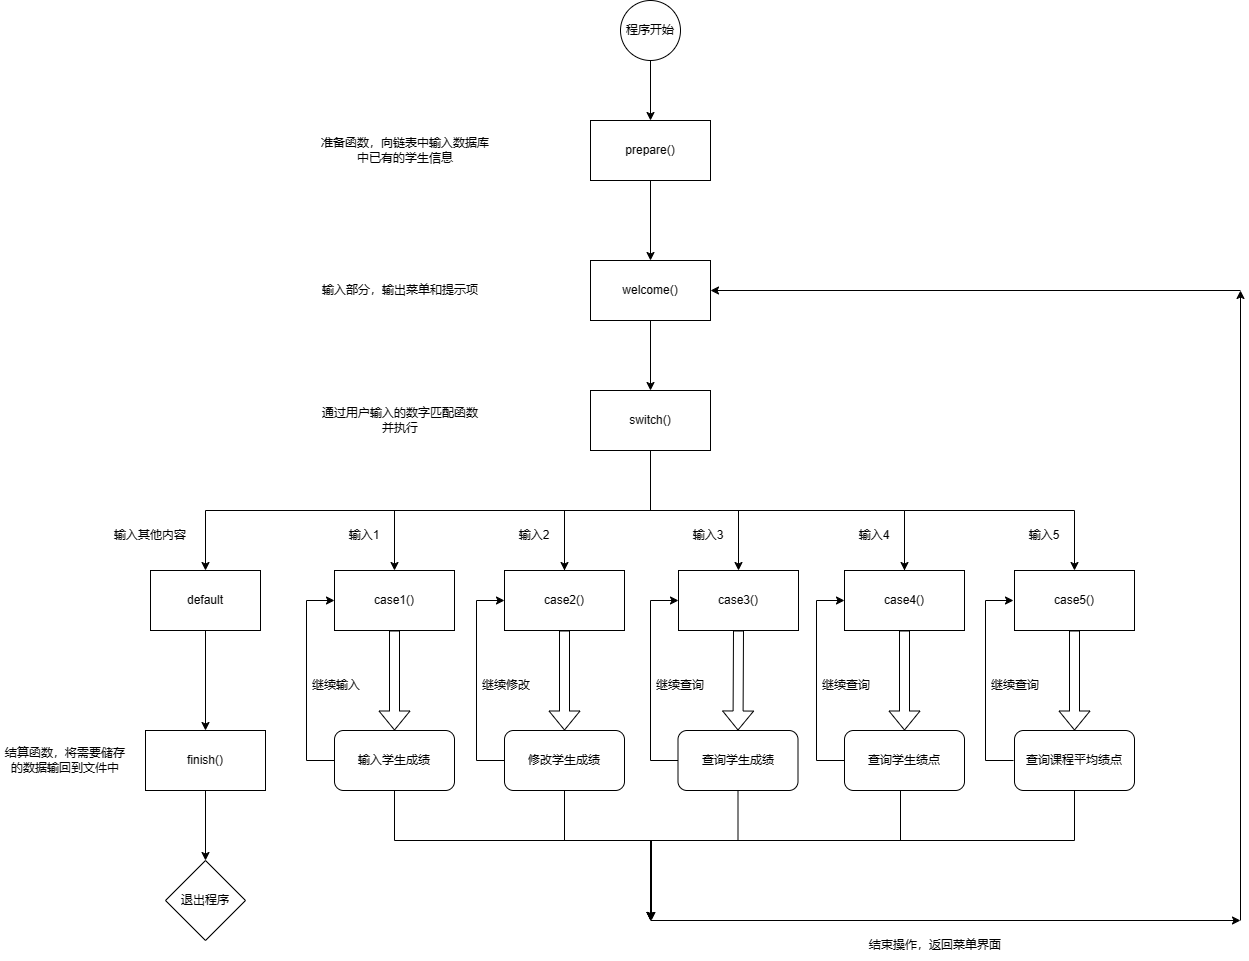
\includegraphics[width = 16cm]{picture1.png}
	\vspace{1cm}
	\caption{学生管理系统的流程图}
\end{figure}

在使用流程方面,当程序开始运行时,首先启动prepare()函数,将文档中的数据加入到链表中,从而实现数据的连续性,防止重复输入
相同数据或数据与先前数据冲突。数据导入完成后,welcome()函数输出菜单,pipei()函数读入用户的输入并匹配到下边具体的函数中
去执行。如果想要退出,可以在菜单页面输入除了选择操作的数字外的任何字符。这将会启动finish()函数,将链表中的数据和其他储存
在全局变量中的需保存数据存储到文件中,等待下次启动时读入。最后,当finish()函数执行完毕,basic类析构函数中的检查将会被激活,
如果链表中的总数据与输入到文件中的数据条数不符,该检查将会输出一条警告,提醒用户有的数据可能丢失。


\section{详细设计}
\subsection{数据结构设计}
在数据结构方面,本系统主要由四个类和两个结构体组成。basic类是做基类的抽象类;people类储存着键盘输入和文件读入
的数据信息,Node类则继承basic类和people类,作为链表的节点。Linkedlist
类则继承basic类,通过操作Node形成链表。每个类之间都是公有继承。student和course则是结构体成员,用于统计链表中的
数据,计算学生的绩点等等。在设计中通过让Node类同时共有继承basic类和people类体现了C++的多继承,同时通过basic中的
纯虚函数wrong()体现了C++的多态性。每个类都至少有四个字段和四个方法,满足了大作业的要求。

\begin{figure}[h!]
	\begin{center}
		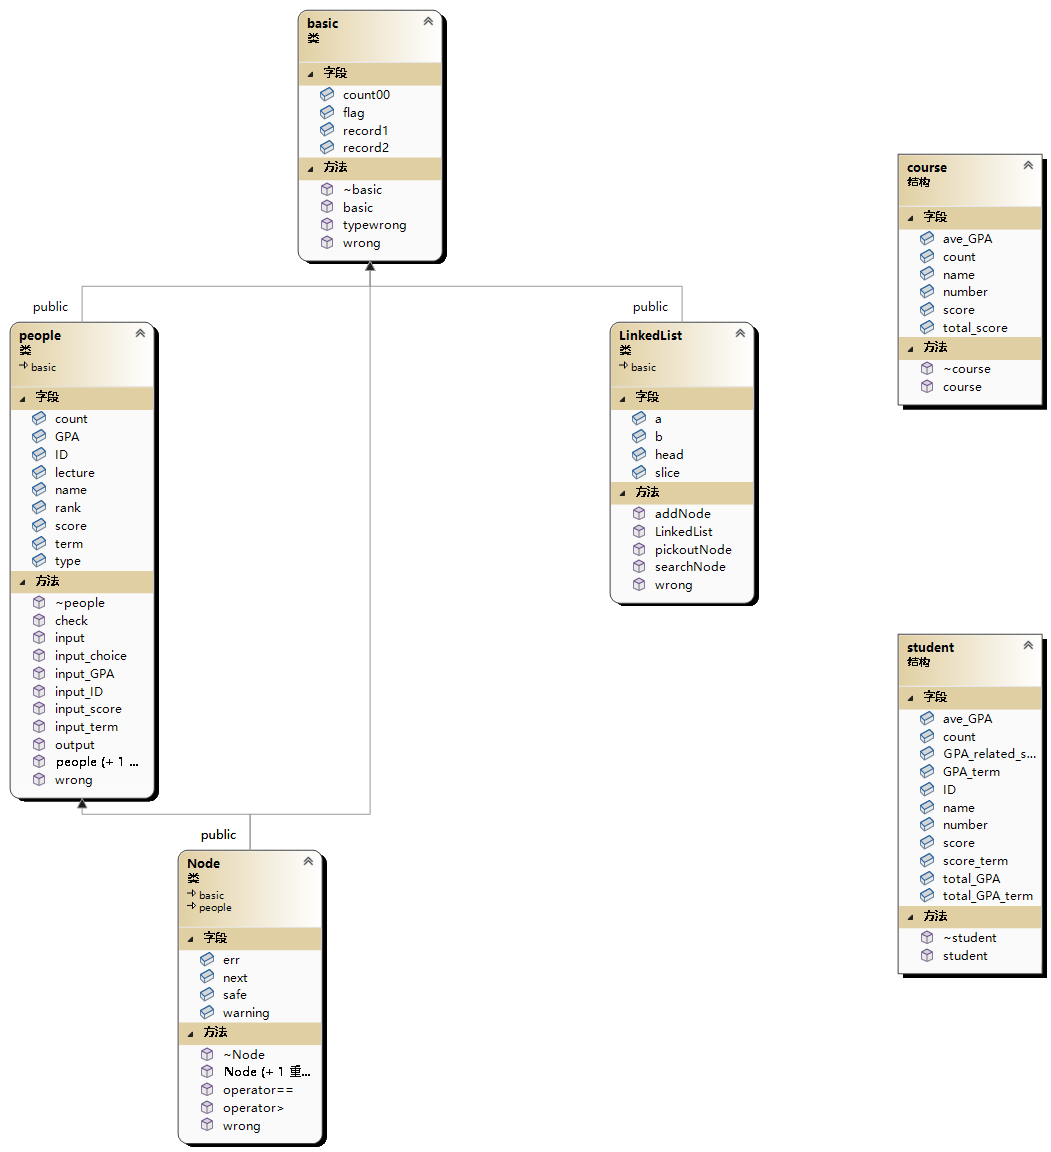
\includegraphics[height = 11cm]{ClassDiagram.png}
		\vspace{1cm}
		\caption{学生管理系统的类视图}
	\end{center}
\end{figure}

用于储存学生信息的结构体中主要有学生姓名,学生学号,学生总学分,学生总学分绩,学生绩点相关学分,学生学期内学分,
学生学期内平均绩点,学生绩点和学生学期内总学分绩这9个数据以及辅助其他函数实现的学生人数计数和学生
报的课程数两个数据。用于储存课程信息的结构体中则有课程名,课程学分数,课程报过的人数,报过该课程的
总人数,课程的总学分绩和课程的平均绩点。这两个结构体并不含有特殊的方法,主要的作用就是在链表中储存
数据。
\subsection{case1()设计}
case1()的作用是将用户从键盘输入的数据存储到链表中。在这一过程中,同时进行的还有链表中数据的排序,数据的
统计与计算绩点。case1()会调用全局函数shuru(),创建一个people类临时变量a,再调用全局变量total的成员函数
addNode将其加入链表。

\vspace{0.5cm}
\begin{figure}[h]
	\begin{center}
		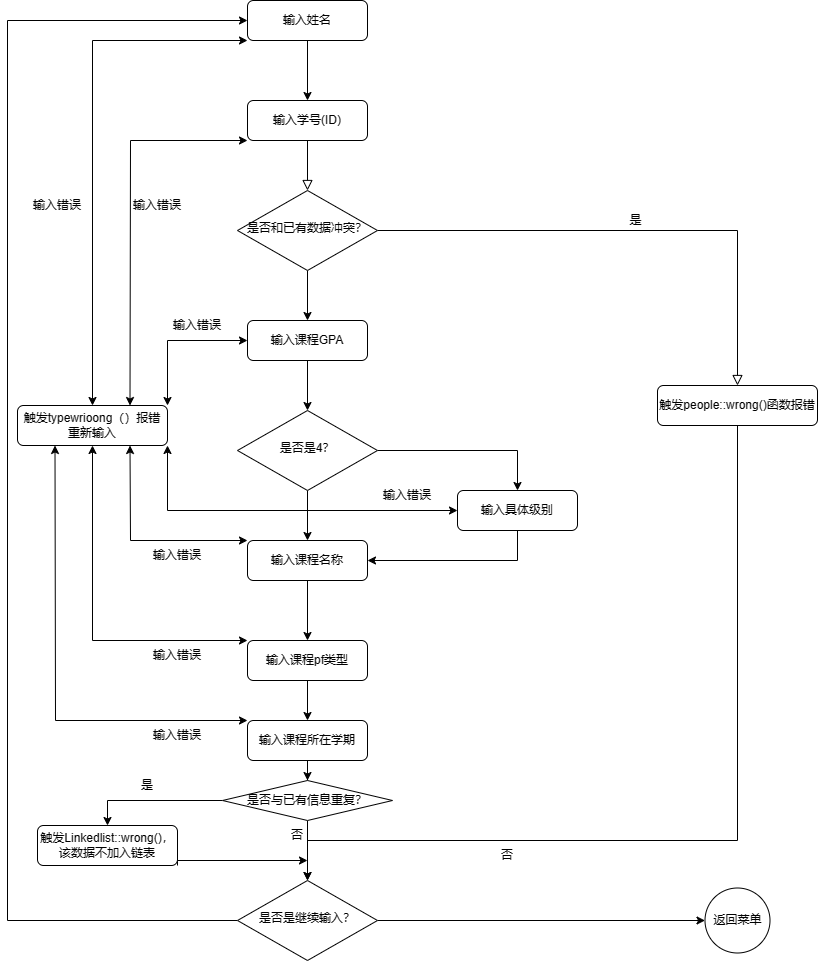
\includegraphics[height = 11cm]{case1.png}
		\vspace{1cm}
		\caption{case1的流程图}
	\end{center}
\end{figure}
\subsection{case2()设计}
case2()的作用是根据输入的学生姓名和学号以及学期找到该学生在特定学期的所有课程记录,然后选择想要更改的记录,并
从四种更改模式中选择一种更改数据,最后询问用户是否继续更改,如果不继续更改的话退出该函数。

\begin{figure}[h]
	\begin{center}
		\vspace{-2cm}
		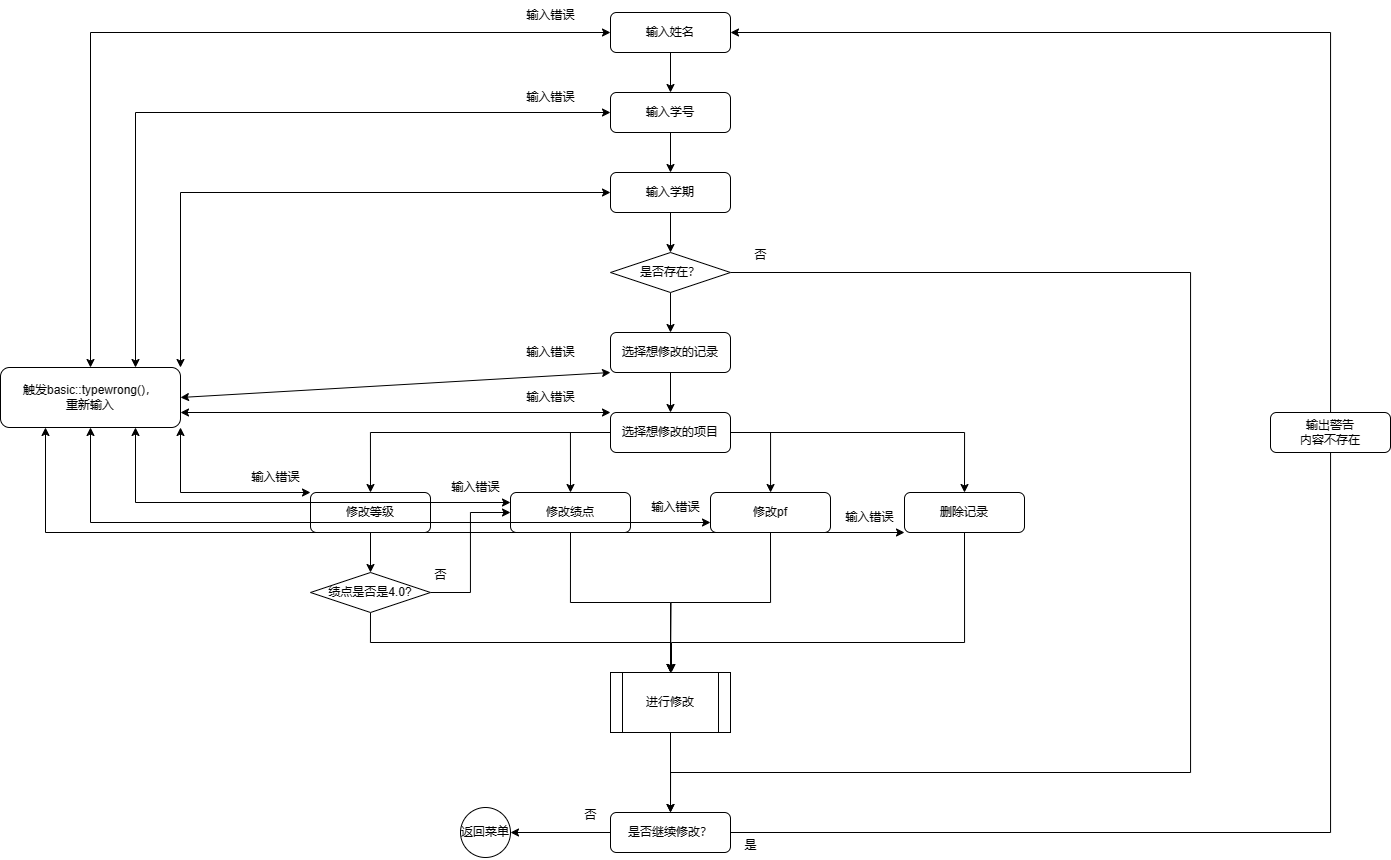
\includegraphics[height = 10cm]{case2.png}
		\vspace{1cm}
		\caption{case2的流程图}
	\end{center}
\end{figure}
\subsection{case3()设计}
case3()的作用是在输入学生的姓名和学号后输出链表中符合该信息的所有信息,相当于输出该学生上过的所有课程及其学分、绩点
、等级、是否记为pf等信息,即打印出该学生的成绩单。

\begin{figure}[h]
	\begin{center}
		\vspace{0.3cm}
		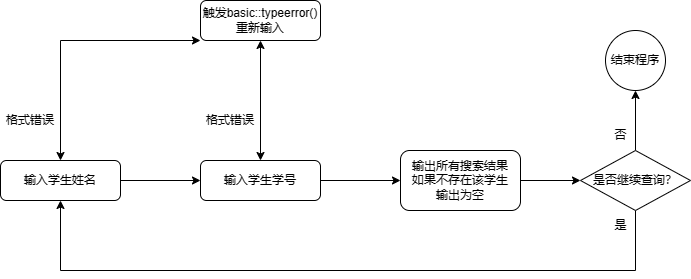
\includegraphics[width = 10cm]{case3.png}
		\vspace{1cm}
		\caption{case3的流程图}
	\end{center}
\end{figure}
\subsection{case4()设计}
case4()的作用是查询学生的绩点。这一函数有两种选择,如果输入“查询全部学生”将会按绩点从高到低输出所有学生的总绩点,也可以只输入一个学生的姓名和学号,
从而查询这个学生的总绩点和每学期的平均绩点。

\begin{figure}[h]
	\begin{center}
		%\vspace{-5cm}
		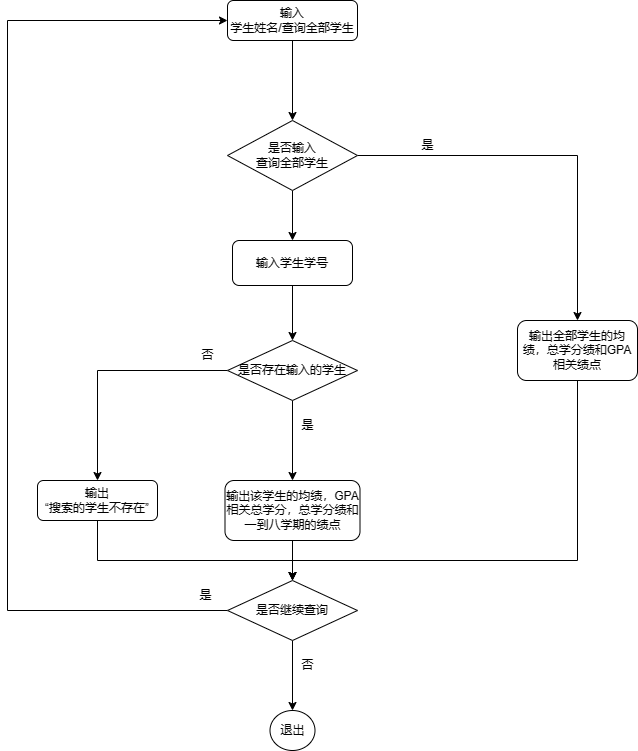
\includegraphics[width = 10cm]{case4.png}
		\vspace{1cm}
		\caption{case4的流程图}
	\end{center}
\end{figure}
\subsection{case5()设计}
case5()的作用是查询课程的平均绩点,这一数值是上过该课的所有学生的绩点的平均值。这一值可以在一定程度上反应课程的给分和
教学情况。用户可以输入课程名来查询特定的课程,也可以直接输入“查询所有课程”,看到课程的平均绩点排名。如果系统没有找到该
课程,将会输出“未查到该课程”提醒用户。
\begin{figure}[h!]
	\begin{center}
		\vspace{0.5cm}
		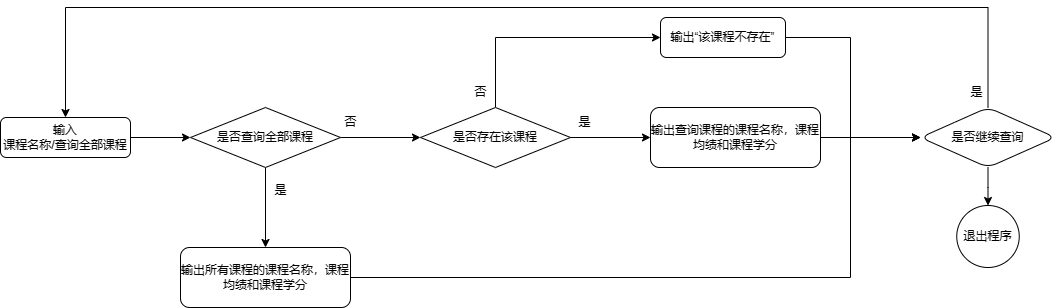
\includegraphics[width = 10cm]{case5.png}
		\vspace{0.5cm}
		\caption{case5的流程图}
	\end{center}
\end{figure}
\newpage

\section{系统调试}
我在写程序的过程中,选择的是写完一个模块测试一个模块的做法。这种做法的好处是可以使得整体上更加清晰,不会出现全部写完后
测试一团乱麻,不知道问题出在哪里。但缺点是在修改比较基础的东西时有可能影响已经测试好的模块,导致其失效,所以每过一段时间
就需要确定之前能正常实现的功能是否还能正常实现。调试过程中,首先出现的问题是输入意料之外的数据时,程序可能会卡死。比如
程序希望读入的是一个int型数据,但输入了一个字符串。为了解决这一问题,我在每一个输入后面都加入了cin.good()的检查,一旦
读入错误,就会马上清除错误状态并忽略输入的错误数据。同时,为了防止过量的数据堆在缓存区里,导致下一次输入读入上一次输入的
数据,每次输入后都会无视缓存区中的剩余数据,同时在数据容易堆积的函数中加入了清楚缓存区。在调试过程中,我发现每次输入完成
后都要返回菜单带来的使用感极差,所以我加入了询问是否要继续输入的环节,这提高了使用的流畅度,改善了输入的手感。在运行中,
我发现我想要赋值的变量并没有被正确的赋值。在多次检查无果后,我选择向学长求助,结果发现是由于我的继承较为混乱,程序实际上
将值赋给了继承来的对象,而非我希望赋值的对象。这也让我开始重新检查我的数据结构。在重新调整了数据结构后,我解决了这一问题。
我还在测试时发现,有的输入明显与事实不符,但仍然可以输入成功,比如两条相同学号但姓名不同的数据,为此我增加了一个数组来储存
学生的姓名与学号的对应关系,同时将这一数据输入到文件中,这解决了可以录入学号相同但姓名不同数据的问题。随着文件存储功能的加入,
我发现了更多的bug。我在文件存储中将文件中数据写入链表的函数调用的是从键盘输入的同一个函数,这个函数在输入成功后会输出“输入成功”
提醒用户,这就使得在文件读入阶段,菜单还未出现时屏幕上就输出了“输入成功”,导致观感很差。我在考虑后增加了一个bool型变量来检测
从文件读入过程是否完成,如果未完成的话,调用加入链表的函数不会输出“输入成功”的提示。我在设计把数据输出到文件的函数中设计了一个
检查程序,在输出函数完成后,如果记录的链表中数据和实际上输出到文件的数据不相符,将会报错,提醒用户可能发生了数据丢失。这个检查
过程和输出过程位于basic类的析构函数中,同时有条件判断确保该输出只会在链表中的数据被全部输入文件后才会起到作用。调试过程很成功,
在正常流程下,该程序确实提醒了用户可能的数据丢失。但如果突然终止调试的话,虽然链表中的数据也没有被全部输入文件,但程序并不会提醒
用户。这就导致如果突然关闭对话框的话,用户无法得知可能的数据丢失,并没有完成我设计时的全部目标。同时,我在基本完成作业后才发现
string类数据非常便捷好用,但我没有使用,这也是我的一个遗憾。但我在整个系统调试的过程中还是学到了很多东西,一些之前看不懂的报错
现在也能看明白了,最大的收获应该是我学会了熟练使用互联网或者向学长提问来获得答案,也知道了如何正确的提出问题。
\section{测试结果与分析}
\subsection{测试用数据}
该程序使用的测试数据如下:

\begin{figure}[h!]
	\begin{center}
		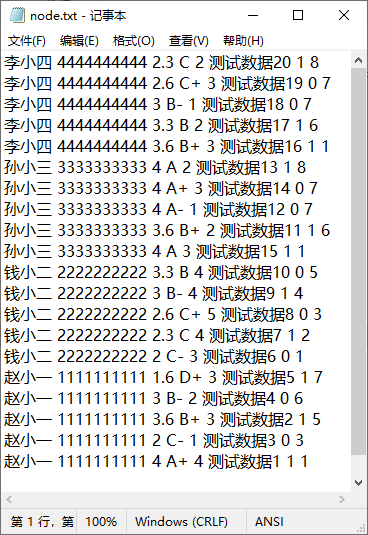
\includegraphics[width = 10cm]{测试数据.png}
		\vspace{0.5cm}
		\caption{测试用学生信息}
	\end{center}
\end{figure}

值得注意的是,测试数据是输入进文本文件的,但学生的学号信息是由该管理系统自动生成的。
同时,学号信息中出现了几条数据并未在测试数据中出现。这是因为这些数据在测试完毕后被手动删除。并不是由于系统的故障产生的。
\begin{figure}
	\begin{center}
		\vspace{-1.5cm}
		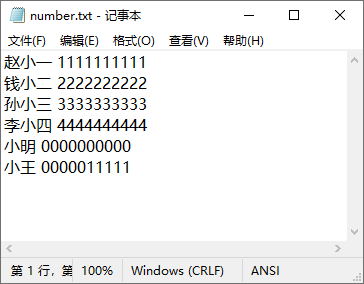
\includegraphics[width = 10cm]{学生信息.png}
		\vspace{0.5cm}
		\caption{学生学号信息}
	\end{center}
\end{figure}
\vspace{5cm}

\subsection{菜单界面}
正常打开程序后,程序将会自动从文件中录入数据,然后显示菜单页面。

\begin{figure}[h!]
	\begin{center}
		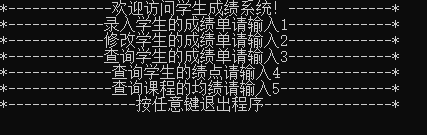
\includegraphics[width = 10cm]{菜单界面.png}
		\caption{菜单页面}
	\end{center}
\end{figure}
%\vspace{-1cm}

在菜单界面输入指定的数字将会进入相应功能,输入其他字符将会退出程序。
\begin{figure}[h!]
	\begin{center}
		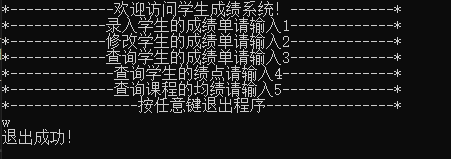
\includegraphics[width = 10cm]{退出.png}
		\caption{退出}
	\end{center}
\end{figure}
\newpage
\subsection{case1()测试图}

正常流程输入下,case1的输入流程不会报错,在所有输入结束后,系统将会输出绿色的“输入成功”,提示用户信息已成功录入,参见图\ref{ref1}。
\begin{figure}[h!]
	\begin{center}
		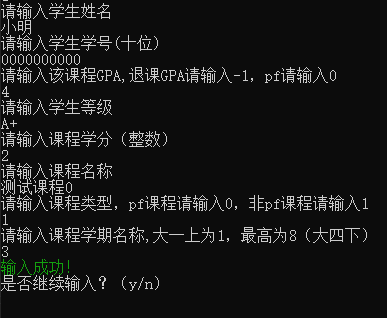
\includegraphics[width = 10cm]{case1 正常输入.png}
		\caption{case1正常输入}
		\label{ref1}
	\end{center}
\end{figure}

如果学生的姓名和学号不匹配,将会触发通用类型错误,系统将会输出红色字体提醒用户,参见图\ref{ref2}。

\begin{figure}[h!]
	\begin{center}
		\vspace{-0.3cm}
		
\includegraphics[width = 10cm]{学生姓名与学号不匹配触发错误.png}
		\caption{学生姓名与学号不匹配时触发错误}
		\label{ref2}
	\end{center}
\end{figure}

如果输入的数据和系统希望得到的数据类型不相符,也将触发通用类型错误,系统将会输出红色字体提醒用户,参见图\ref{ref3}。

\begin{figure}[h!]
	\begin{center}
		\vspace{-0.3cm}
		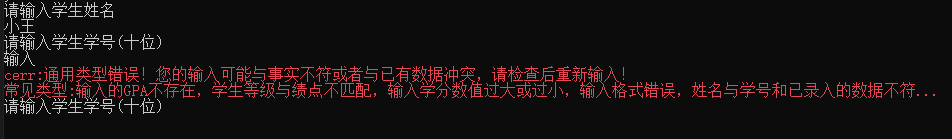
\includegraphics[width = 10cm]{输入不相符的数据时发出警告.png}
		\caption{输入不相符的数据时发出警告}
		\label{ref3}
	\end{center}
\end{figure}
\newpage

\subsection{case2()测试图}


正常流程输入下,case2的输入流程不会报错。在输入学生姓名,学生学号和想要修改的学期后,系统将会输出所有符合条件的课程记录,将会进入case2的菜单
页面。在菜单页面可以选择修改学生等级,学生绩点,课程pf或者直接删除该记录。修改的记录允许与上次的相同。在所有输入结束后,系统将会输出绿色的“输
入成功”,提示用户已成功修改。

修改学生等级参见图\ref{ref4},修改学生绩点参见图\ref{ref5},修改课程pf参见图\ref{ref6},删除学生成绩参见图\ref{ref7}。

\begin{figure}[h!]
	\begin{center}
		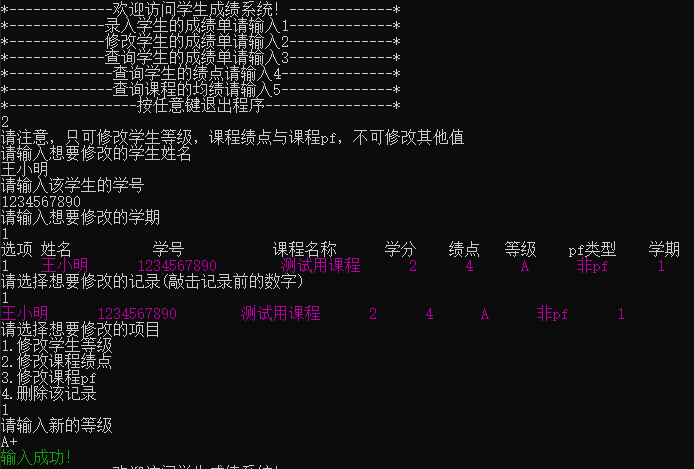
\includegraphics[width = 10cm]{修改学生等级.png}
		\caption{修改学生等级}
		\label{ref4}
		\end{center}
\end{figure}

\begin{figure}[h!]
	\begin{center}
		\vspace{-0.3cm}
		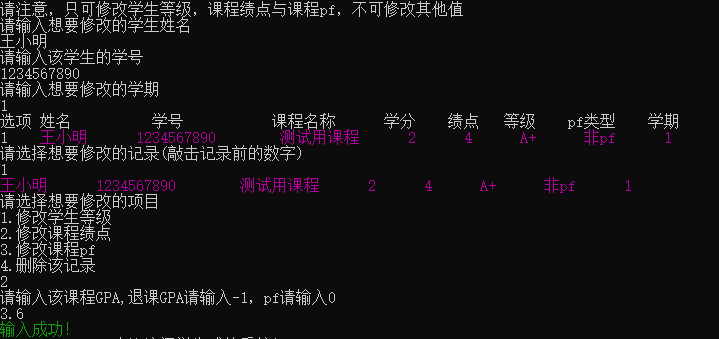
\includegraphics[width = 10cm]{修改学生绩点.png}
		\caption{修改学生绩点}
		\label{ref5}
	\end{center}
\end{figure}

\newpage

\begin{figure}[h!]
	\begin{center}
		\vspace{-0.3cm}
		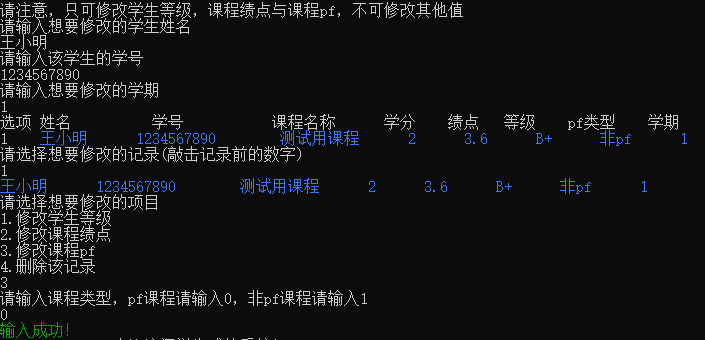
\includegraphics[width = 10cm]{修改课程pf.png}
		\caption{修改课程pf}
		\label{ref6}
	\end{center}
\end{figure}

\begin{figure}[h!]
	\begin{center}
		\vspace{-0.3cm}
		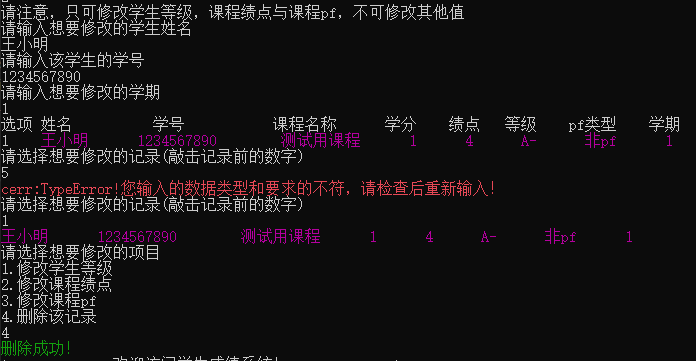
\includegraphics[width = 10cm]{case2 成功删除学生成绩.png}
		\caption{删除学生成绩}
		\label{ref7}
	\end{center}
\end{figure}

应当注意的是,由于绩点和等级的对应性,只有特定的等级可以修改绩点。因此,如果学生的绩点不是4.0,系统回发出
警告并跳转到修改绩点处,参见图\ref{ref8}。

\begin{figure}[h!]
	\begin{center}
		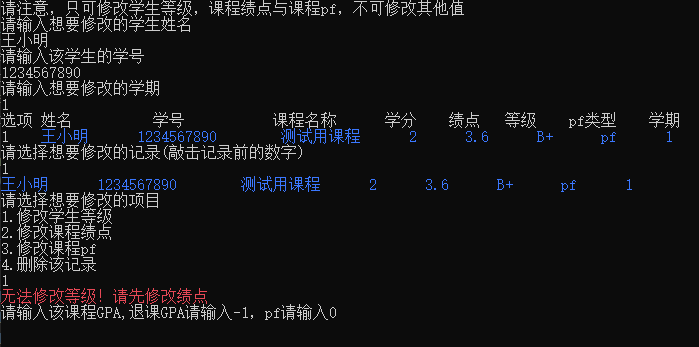
\includegraphics[width = 10cm]{无法修改学生等级.png}
		\caption{无法修改学生等级}
		\label{ref8}
	\end{center}
\end{figure}

如果系统未找到想要修改学生的记录,将会输出红色字体警告用户不存在该学生的记录,参见图\ref{ref9}。
\newpage
\begin{figure}[h!]
	\begin{center}
		\vspace{-0.3cm}
		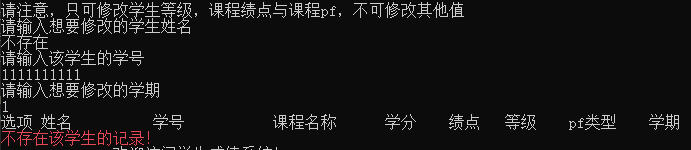
\includegraphics[width = 10cm]{case2 不存在该学生的记录.png}
		\caption{不存在该学生的记录}
		\label{ref9}
	\end{center}
\end{figure}

如果选择要修改的记录时,选择的记录与提供的所有选项都不相符,将会触发TypeError,系统将会输出红色字体提醒用户,参见图\ref{ref10}。

\begin{figure}[h!]
	\begin{center}
		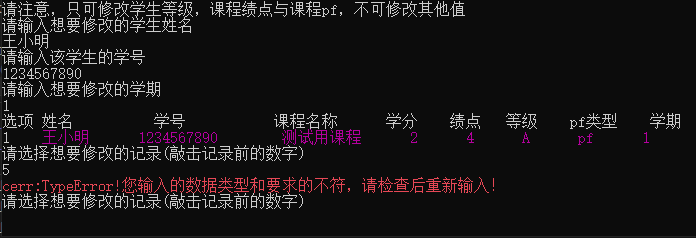
\includegraphics[width = 10cm]{case2 输入类型错误.png}
		\caption{输入有误的选项}
		\label{ref10}
	\end{center}
\end{figure}

\subsection{case3()测试图}
case3()操作时需要输入想查询学生的姓名和学号, 系统会将于此数据对应的所有数据排序输出。排序顺序为学期,课程,GPA,等级和学分依次降序排列,
参见图\ref{ref11}。

\begin{figure}[h!]
	\begin{center}
		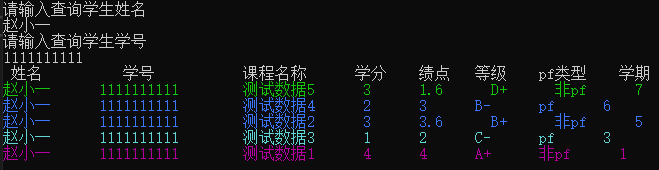
\includegraphics[width = 10cm]{case3 赵小一.png}
		\caption{赵小一成绩单}
		\label{ref11}
	\end{center}
\end{figure}

在完成一次输出后,系统将会询问是否继续输出,即允许用户连续查询成绩单,参见图\ref{ref12}、图\ref{ref13}。
\newpage
\begin{figure}[h!]
	\begin{center}
		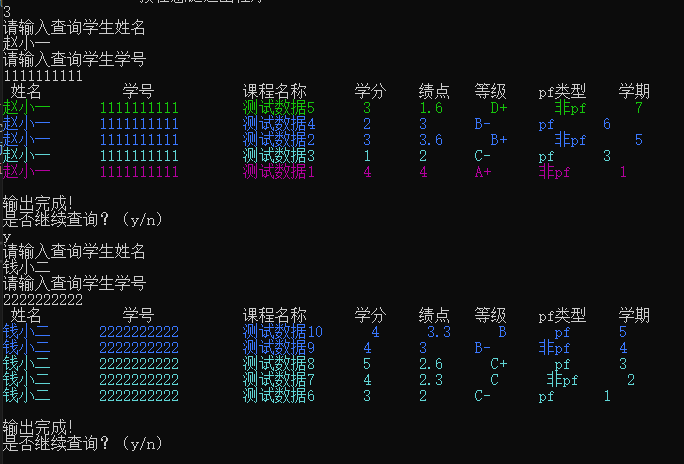
\includegraphics[width = 10cm]{case3 赵小一+钱小二 连续输出.png}
		\caption{赵小一+钱小二 连续输出}
		\label{ref12}
	\end{center}
\end{figure}

\begin{figure}[h!]
	\begin{center}
		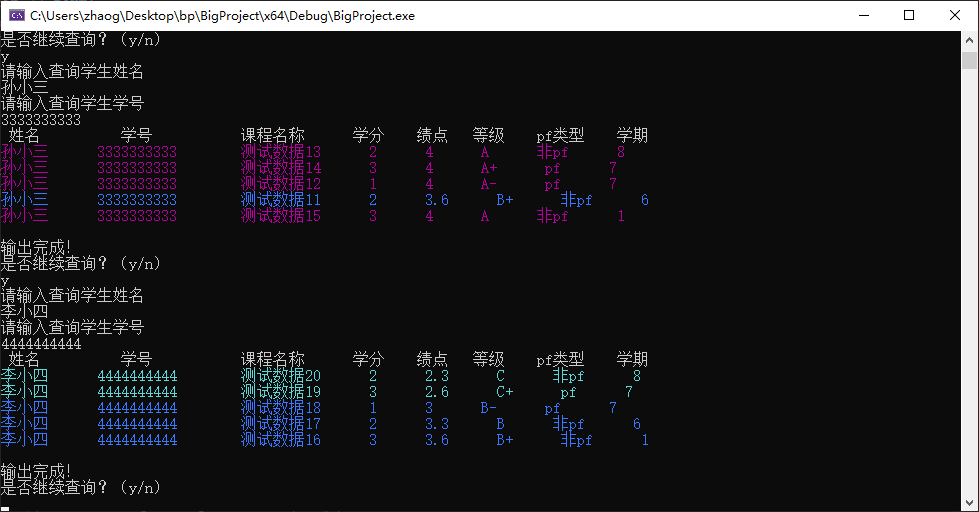
\includegraphics[width = 10cm]{case3 钱小三+李小四.png}
		\caption{钱小三+李小四 连续输出}
		\label{ref13}
	\end{center}
\end{figure}

如果用户输入不存在的学生或输入的学生姓名与学号不匹配,系统将不会输出任何课程记录,,参见图\ref{ref14}、图\ref{ref15}。
\newpage
\begin{figure}[h!]
	\begin{center}
		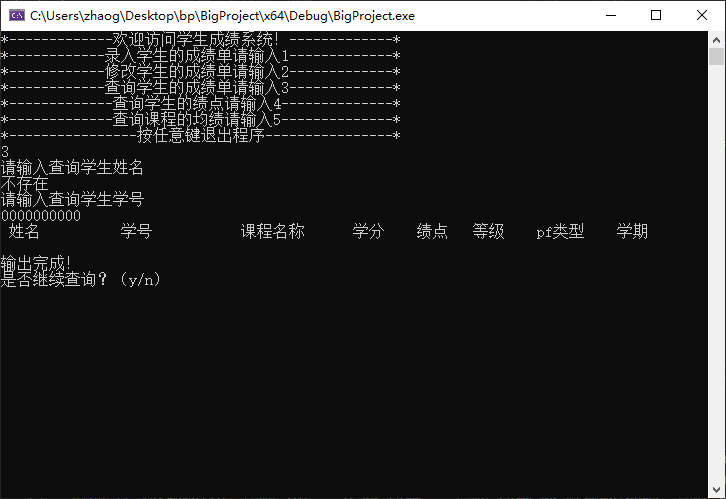
\includegraphics[width = 10cm]{case3 不存在.png}
		\caption{输入不存在的学生}
		\label{ref14}
	\end{center}
\end{figure}

\begin{figure}[h!]
	\begin{center}
		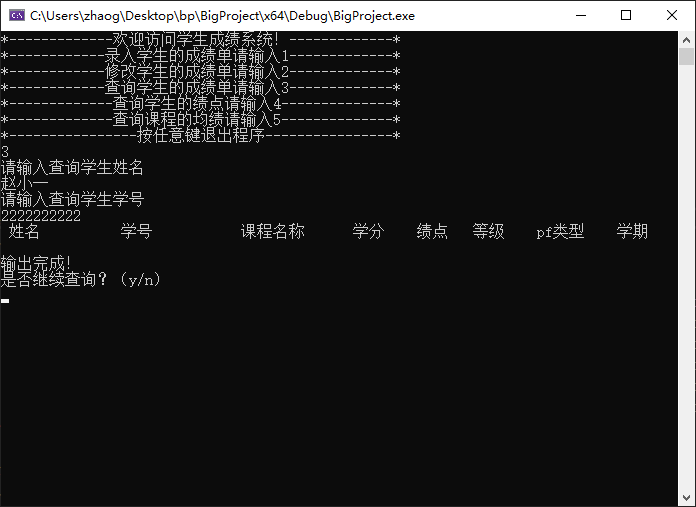
\includegraphics[width = 10cm]{case3 不存在2.png}
		\caption{输入错误的学生姓名和学号关系}
		\label{ref15}
	\end{center}
\end{figure}

\subsection{case4()测试图}
case4()有两个可选模式,用户可以选择查询所有学生的成绩绩点或查询单个学生的绩点。

如果输入“查询全部学生”,系统将会输出所有学生的总绩点,排序顺序为学期,课程,GPA,等级和学分依次降序排列;
如果输入想查询学生的姓名和学号,将会输出该学生的总绩点,总学分绩,GPA相关总学分和每学期的平均绩点;
在输出完成后,系统也会询问用户是否继续查询,参见图\ref{ref16}。
\newpage
\begin{figure}[h!]
	\begin{center}
		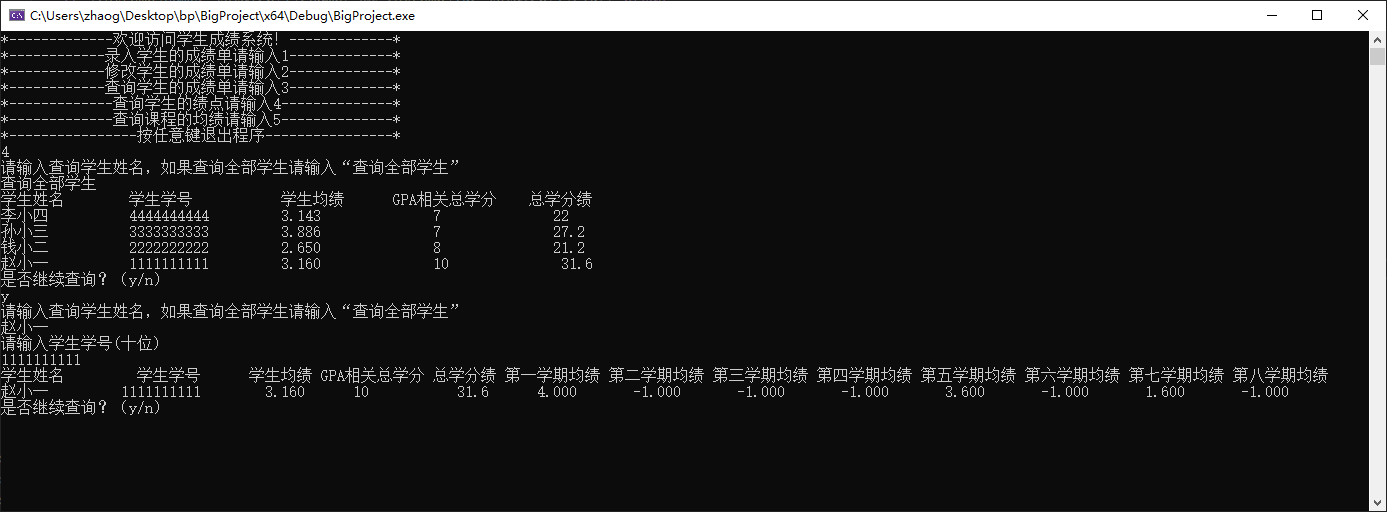
\includegraphics[width = 10cm]{case4 查询全部学生+赵小一 连续输出.png}
		\caption{查询全部学生\&单独查询赵小一}
		\label{ref16}
	\end{center}
\end{figure}

同时,如果输入不存在的人,系统将会用红色字体警告查询的人不存在,参见图\ref{ref17}。

\begin{figure}[h!]
	\begin{center}
		
\includegraphics[width = 10cm]{case4 输入不存在的人.png}
		\caption{输入不存在的人}
		\label{ref17}
	\end{center}
\end{figure}

\subsection{case5()测试图}
case5()有两个可选模式,用户可以选择查询所有课程的平均绩点或查询单个课程的平均绩点。
两者的输出内容都是课程的名称,平均绩点和学分。参见图\ref{ref18}、图\ref{ref19}。

\begin{figure}[h!]
	\begin{center}
		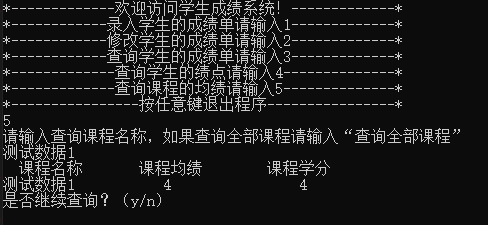
\includegraphics[width = 10cm]{查询单个课程.png}
		\caption{查询单个课程}
		\label{ref18}
	\end{center}
\end{figure}
\newpage
\begin{figure}[h!]
	\begin{center}
		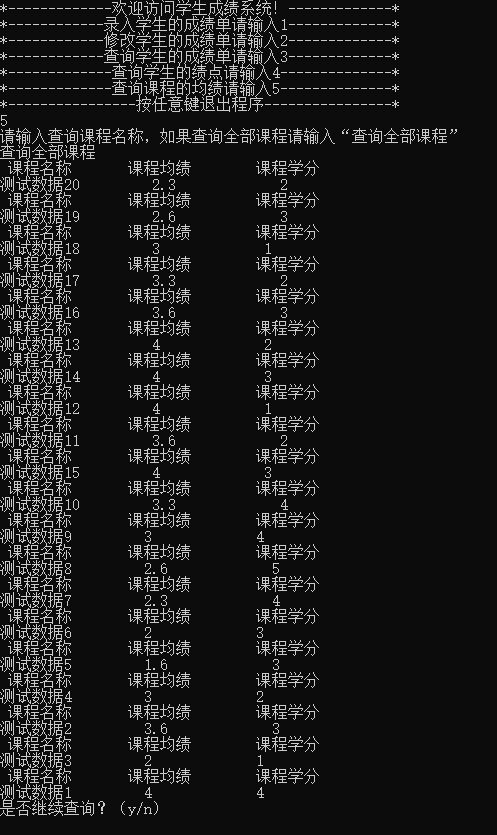
\includegraphics[width = 10cm]{查询全部课程.png}
		\caption{查询全部课程}
		\label{ref19}
	\end{center}
\end{figure}

如果用户输入的课程不存在,系统将会输出红色字体警告用户课程不存在,参见图\ref{ref20}
\newpage
\begin{figure}[h!]
	\begin{center}
		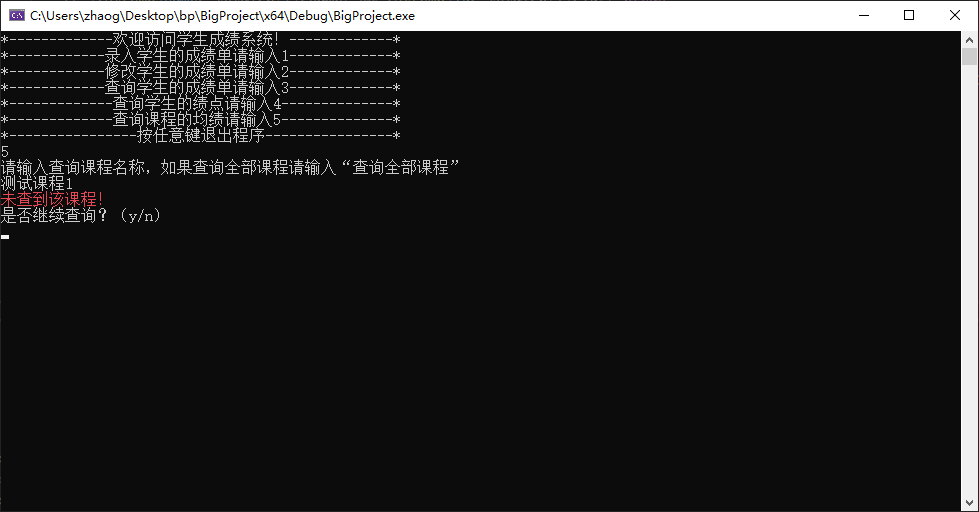
\includegraphics[width = 10cm]{case5 不存在课程.png}
		\caption{输入不存在的课程}
		\label{ref20}
	\end{center}
\end{figure}

\section{总结}
从这次程设大作业中,我学到了很多东西。对我来说,这次大作业不仅仅给了我全面练习过去一年中所学的知识的机会,也让我学会了如何上手
去写一个相对较大的项目。在这个过程中,我学会了如何清晰准确的表达出自己的疑问,学会了如何从互联网上寻找答案。在编程的亲身体验中,
我也体会到了写注释和版本控制的重要性。这次程设大作业不仅仅是对我所学知识的一次应用,更是一次全新的学习的过程。

\newpage

\appendix
\section*{附录1:源程序清单}
\addcontentsline{toc}{section}{附录1:源程序清单}    %可以不进行编目,所以没有前面的A
\vspace{1cm}
\begin{lstlisting}[style = {cppstyle}]
	#include<iostream>
	#include<cstring>
	#include<windows.h>
	#include<fstream>
	#include<iomanip>
	
	HANDLE hConsole = GetStdHandle(STD_OUTPUT_HANDLE);
	#pragma warning(disable:4996)
	using namespace std;
	
	//****************************************************下面开始是类****************************************************//
	
	
	//基本类,里面装有基本的函数方法
	
	class basic
	{
	public:
		basic(){}
		~basic(){
		}
		virtual void wrong() = 0;//为其类中的报错函数提供接口
		//较为通用的输入报错函数
		static void typewrong()
		{
			SetConsoleTextAttribute(hConsole, FOREGROUND_RED | FOREGROUND_INTENSITY);
			cout << "cerr:TypeError!您输入的数据类型和要求的不符,请检查后重新输入!" << endl;
			SetConsoleTextAttribute(hConsole, FOREGROUND_RED | FOREGROUND_GREEN | FOREGROUND_BLUE);
		}
		static int count00;//记录现有的所有学生学号与姓名数据数
		static char record1[10000][30];//用于输入学生姓名
		static char record2[10000][11];//用于输入学生学号
		static bool flag;//用于确认已经完成数据读入,防止数据读入时输出
	};
	
	int basic::count00 = 0;
	char basic::record1[10000][30];
	char basic::record2[10000][11];
	bool basic::flag = false;
	
	
	//学生类,里面继承了学生单门课程的信息
	class people:virtual public basic
	{
	public:
		people() {};
		~people() {};
		void wrong()
		{
			SetConsoleTextAttribute(hConsole, FOREGROUND_RED | FOREGROUND_INTENSITY);
			cout << "cerr:通用类型错误!您的输入可能与事实不符或者与已有数据冲突,请检查后重新输入!" << endl;
			cout << "常见类型:输入的GPA不存在,学生等级与绩点不匹配,输入学分数值过大或过小,输入格式错误,姓名与学号和已录入的数据不符..." << endl;
			SetConsoleTextAttribute(hConsole, FOREGROUND_RED | FOREGROUND_GREEN | FOREGROUND_BLUE);
		}
		people(const people &data) {
			this->count = data.count;
			this->score = data.score;
			strcpy(this->name, data.name);
			strcpy(this->lecture, data.lecture);
			this->GPA = data.GPA;
			strcpy(this->rank, data.rank);
			this->type = data.type;
			this->term = data.term;
			strcpy(this->ID, data.ID);
		}
	
		//从键盘输入学生绩点并判断等级类型 
		void input_GPA()
		{
	
			cout << "请输入该课程GPA,退课GPA请输入-1,pf请输入0" << endl;
			cin >> GPA;
			while (!cin.good()) { 
			cin.clear();
			cin.ignore(10000, '\n');
			typewrong();
			cout << "请输入该课程GPA,退课GPA请输入-1,pf请输入0" << endl;
			cin >> GPA;
			}
			if (GPA != 4.0 && GPA != 3.6 && GPA != 3.3 && GPA != 3.0 && GPA != 2.6 && GPA != 2.3 && GPA != 2.0 && GPA != 1.6 && GPA != 1.0 && GPA != 0.0 && GPA != -1) {
				wrong();
				input_GPA();
			}
			else {
				if (GPA == -1) { strcat(rank, "W"); }
				if (GPA == 0.0) { strcat(rank, "F"); }
				if (GPA == 1.0) { strcat(rank, "D-"); }
				if (GPA == 1.3) { strcat(rank, "D"); }
				if (GPA == 1.6) { strcat(rank, "D+"); }
				if (GPA == 2.0) { strcat(rank, "C-"); }
				if (GPA == 2.3) { strcat(rank, "C"); }
				if (GPA == 2.6) { strcat(rank, "C+"); }
				if (GPA == 3.0) { strcat(rank, "B-"); }
				if (GPA == 3.3) { strcat(rank, "B"); }
				if (GPA == 3.6) { strcat(rank, "B+"); }
				if (GPA == 4.0) {
					int flag = 0;
					while (!flag) {
						flag = 1;
						cout << "请输入学生等级" << endl;
						cin >> rank;
						while (!cin.good())
							{
								cin.clear();
								cin.ignore(10000, '\n');
								typewrong();
								cout << "请输入该课程GPA,退课GPA请输入-1,pf请输入0" << endl;
								cin >> rank;
							}
						if (strcmp(rank, "A") * strcmp(rank, "A-") * strcmp(rank, "A+")) {
							wrong();
							flag = 0;
						}
					}
				}
			}
		}
	
		//从键盘输入课程学分
		void input_score()
		{
			cout << "请输入课程学分(整数)" << endl;
			cin >> score;
			while (!cin.good()) {
				cin.clear();
				cin.ignore(10000, '\n');
				typewrong();
				cin >> score;
			}
			if (score < 0 || score > 20 || score < 0) {
				wrong();
				input_score();
			}
		}
	
		//从键盘输入课程pf类型
		void input_choice() {
			cout << "请输入课程类型,pf课程请输入0,非pf课程请输入1" << endl;
			cin >> type;
			while (!cin.good()) {
				typewrong();
				cin.clear();
				cin.ignore(10000, '\n');
				cin >> type;
			}
			while (type != 0 && type != 1) { 
				wrong();
				cin >> type;
			}
		}
	
		void input_term() {
			cout << "请输入课程学期名称,大一上为1,最高为8(大四下)" << endl;
			cin >> term;
			while (!cin.good()) {
				typewrong();
				cin.clear();
				cin.ignore(10000, '\n');
				cin >> term;
			}
			if (term != 1 && term != 2 && term != 3 && term != 4 && term != 5 && term != 6 && term != 7 && term != 8) { wrong(); input_choice(); }
		}
	
		void input_ID() {
			cout << "请输入学生学号(十位)" << endl;
			cin >> ID;
			while (!cin.good()) {
				cin.clear();
				cin.ignore(10000, '\n');
				typewrong();
				cin >> ID;
			}
			if (strlen(ID) - 10) {
				wrong();
				input_ID();
			}
		}
	
		bool check()
		{
			for (int i = 0; i < count00; i++)
			{
				if (strcmp(record1[i], name) == 0 && strcmp(record2[i], ID) == 0)
				{
					count--;
					return false;
				}
			}
			strcat(record1[count00], name);
			strcat(record2[count00], ID);
			for (int i = 0; i < count00; i++)
			{
				if ((strcmp(record1[i], name) != 0 && strcmp(record2[i], ID) == 0))
				{
					*record1[count00] = { 0 };
					*record2[count00] = { 0 };
					return true;
				}
			}
			return false;
		}
		//输入函数,在用户选择1后输出指示,引导用户输入信息     
		int input()
		{
			cout << "请输入学生姓名" << endl;
			cin >> name;
			while (!cin.good()) {
				cin.clear();
				cin.ignore(10000, '\n');
				typewrong();
				cin >> name;
			}
			cin.clear();
			cin.ignore(10000, '\n');
			input_ID();
			cin.clear();
			cin.ignore(10000, '\n');
			if (check()) {
				*name = { 0 };
				*ID = { 0 };
				wrong();
				return 0;
			}
			else
			{
				count00++;
				input_GPA();
				cin.clear();
				cin.ignore(10000, '\n');
				input_score();
				cin.clear();
				cin.ignore(10000, '\n');
				cout << "请输入课程名称" << endl;
				cin >> lecture;
				while (!cin.good()) {
					cin.clear();
					cin.ignore(10000, '\n');
					typewrong();
	
					cin >> lecture;
				}
				cin.clear();
				cin.ignore(10000, '\n');
				input_choice();
				cin.clear();
				cin.ignore(10000, '\n');
				input_term();
				cin.clear();
				cin.ignore(10000, '\n');
				return 1;
			}
		}
		//输出函数,查询时输出储存好的信息。
		void output() { 
			if (GPA == 4)
			{
				SetConsoleTextAttribute(hConsole, FOREGROUND_RED | FOREGROUND_BLUE | FOREGROUND_INTENSITY); 
				cout << name;
				cout << "      " << ID << "        ";
				cout << lecture;
				cout << "      " << score << "      " << GPA << "      ";
				cout << rank;
				if (type) { cout << "      " << "非pf" << "      " << term << endl; }
				else { cout << "      " << "pf" << "      " << term << endl; }
				SetConsoleTextAttribute(hConsole, FOREGROUND_RED | FOREGROUND_GREEN | FOREGROUND_BLUE);
			}
			if (GPA < 4 && GPA >= 3)
			{
				SetConsoleTextAttribute(hConsole, FOREGROUND_BLUE | FOREGROUND_INTENSITY);
				cout << name;
				cout << "      " << ID << "        ";
				cout << lecture;
				cout << "      " << score << "      " << GPA << "      ";
				cout << rank;
				if (type) { cout << "      " << "非pf" << "      " << term << endl; }
				else { cout << "      " << "pf" << "      " << term << endl; }
				SetConsoleTextAttribute(hConsole, FOREGROUND_RED | FOREGROUND_GREEN | FOREGROUND_BLUE);
			}
			if (GPA < 3 && GPA >=2)
			{
				SetConsoleTextAttribute(hConsole, FOREGROUND_GREEN | FOREGROUND_BLUE | FOREGROUND_INTENSITY);
				cout << name;
				cout << "      " << ID << "        ";
				cout << lecture;
				cout << "      " << score << "      " << GPA << "      ";
				cout << rank;
				if (type) { cout << "      " << "非pf" << "      " << term << endl; }
				else { cout << "      " << "pf" << "      " << term << endl; }
				SetConsoleTextAttribute(hConsole, FOREGROUND_RED | FOREGROUND_GREEN | FOREGROUND_BLUE);
			}
			if (GPA < 2 && GPA > 0)
			{
				SetConsoleTextAttribute(hConsole, FOREGROUND_GREEN | FOREGROUND_INTENSITY);
				cout << name;
				cout << "      " << ID << "        ";
				cout << lecture;
				cout << "      " << score << "      " << GPA << "      ";
				cout << rank;
				if (type) { cout << "      " << "非pf" << "      " << term << endl; }
				else { cout << "      " << "pf" << "      " << term << endl; }
				SetConsoleTextAttribute(hConsole, FOREGROUND_RED | FOREGROUND_GREEN | FOREGROUND_BLUE);
			}
			if (GPA <= 0 )
			{
				cout << name;
				cout << "      " << ID << "        ";
				cout << lecture;
				cout << "      " << score << "      " << GPA << "      ";
				cout << rank;
				if (type) { cout << "      " << "非pf" << "      " << term << endl; }
				else { cout << "      " << "pf" << "      " << term << endl; }
			}
		}	
	
		static int count;  //人数计数
		int score = -1; //学分
		char name[30] = {"ZanderZhao"};//姓名
		char lecture[30] = {"摸鱼课导论"};//课程名
		double GPA;//绩点
		char rank[3] = {};//等级
		int type = 1;//是否pf
		int term; //学期
		char ID[11]; //学生学号
	};
	int people::count = 0;
	
	//****************************************************下面开始是存储数据的结构体****************************************************//
	
	//课程类,方便后面的课程排序
	struct course
	{
	public:
		course() {};
		~course() {};
		static int count; //课程库里一共有几条课程
		char name[30] = {"摸鱼课导论"}; // 课程名
		double score = 0.0; // 学分数
		int number = 0; // 报过的人数
		double total_score = 0; //总学分绩
		//int type; // 暂时去掉,因为pf机制的存在,课程本身的pf已经不重要了    重新更改,这个现在是是否手动置为pf
		double ave_GPA; //平均分数
	};
	int course::count = 0;
	
	//学生类,用来记录学生均绩,从而方便后面排序
	struct student
	{
	public:
		student() {};
		~student() {};
		static int count; //学生人数计数
		char name[30] = { "nullptr" }; //学生姓名
		char ID[11] = { "0000000000" };//学生学号
		int score = 0; //学生总学分
		double total_GPA = 0; //学生总学分绩
		double GPA_related_score = 0; //学生绩点相关学分
		double ave_GPA = 0;  //学生总绩点
		double score_term[8] = { 0,0,0,0,0,0,0,0 }; //学生学期内总学分
		double GPA_term[8] = { -1,-1,-1,-1,-1,-1,-1,-1 }; //学生学期内平均绩点
		double total_GPA_term[8] = { 0,0,0,0,0,0,0,0 }; //学生学期内总绩点
		int number = 0; //学生报的课程数
	};
	int student::count = 0;
	
	//****************************************************下面开始是链表****************************************************//
	
	// 节点类
	class Node :virtual public basic, public people
	{
	public:
		Node() {};
		~Node() {};
		Node* next = NULL;
		static int safe;
		static int warning;
		char err[40] = { "cerr:警告!调用了错误的函数实例!" };
		bool operator>(const Node& temp) {
		if (strcmp(ID,temp.ID) > 0) { return 1; }
		else if (strcmp(ID, temp.ID) == 0 && term > temp.term) { return 1; }
		else if (strcmp(ID, temp.ID) == 0 && term == temp.term && strcmp(name, temp.name) > 0) { return 1; }
		else if (strcmp(ID, temp.ID) == 0 && term == temp.term && strcmp(name, temp.name) == 0 && strcmp(lecture, temp.lecture) > 0) { return 1; }
		else if (strcmp(ID, temp.ID) == 0 && term == temp.term && strcmp(name, temp.name) == 0 && strcmp(lecture, temp.lecture) == 0 && GPA > temp.GPA) { return 1; }
		else if (strcmp(ID, temp.ID) == 0 && term == temp.term && strcmp(name, temp.name) == 0 && strcmp(lecture, temp.lecture) == 0 && GPA == temp.GPA && strcmp(rank, temp.rank) > 0) { return 1; }
		else if (strcmp(ID, temp.ID) == 0 && term == temp.term && strcmp(name, temp.name) == 0 && strcmp(lecture, temp.lecture) == 0 && GPA == temp.GPA && strcmp(rank, temp.rank) == 0 && score > temp.score) { return 1; }
		else if (strcmp(ID, temp.ID) == 0 && term == temp.term && strcmp(name, temp.name) == 0 && strcmp(lecture, temp.lecture) == 0 && GPA == temp.GPA && strcmp(rank, temp.rank) == 0 && score == temp.score && type > temp.type) { return 1; }
		else return 0;
		}	
		void wrong()
		{
			SetConsoleTextAttribute(hConsole, FOREGROUND_RED | FOREGROUND_INTENSITY);
			cout << err << endl;
			SetConsoleTextAttribute(hConsole, FOREGROUND_RED | FOREGROUND_GREEN | FOREGROUND_BLUE);
		}
		bool operator==(const Node& temp) {
		if (!strcmp(ID, temp.ID) && strcmp(name, temp.name) == 0 && strcmp(lecture, temp.lecture) == 0 && GPA == temp.GPA && strcmp(rank, temp.rank) == 0 && score == temp.score && type == temp.type && temp.term == term) { return 1; }
		else return 0;
	}
	
		Node(people& data) {
			this->count = data.count;
			this->score = data.score;
			strcpy(this->name,data.name);
			strcpy(this->lecture, data.lecture);
			this->GPA = data.GPA;
			strcpy(this->rank, data.rank);
			this->type = data.type;
			this->term = data.term;
			strcpy(this->ID, data.ID);
			this->next = nullptr;
		}
	};
	int Node::safe = 0;
	int Node::warning = 0;
	
	
	
	
	
	// 链表类
	class LinkedList :public basic {
	public:
		Node* head;
		course a[20000];
		student b[100000];
		Node* slice[100] = { NULL };
		LinkedList() {
			head = nullptr;
		}
		void wrong()
		{
			SetConsoleTextAttribute(hConsole, FOREGROUND_RED | FOREGROUND_INTENSITY);
			cout << "该条数据已经存在!" << endl;
			SetConsoleTextAttribute(hConsole, FOREGROUND_RED | FOREGROUND_GREEN | FOREGROUND_BLUE);
			count00--;
		}
		// 添加节点函数 
		void addNode(people data) {
			Node* newNode = new Node(data);
			Node::safe++;
			int i = 1;
			int flag = 1;
			char mid[30];
			double middle;
			char mid_id[11];
			if (head == nullptr) {
				head = newNode;
				if (basic::flag)
				{
					SetConsoleTextAttribute(hConsole, FOREGROUND_GREEN);
					cout << "输入成功!" << endl;
					SetConsoleTextAttribute(hConsole, FOREGROUND_RED | FOREGROUND_GREEN | FOREGROUND_BLUE);
				}
			}
			else {
				Node* current = head;
	
				//链表插入顺序控制
	
				if (*newNode == *current) {
					if (basic::flag) wrong();
					i = 0;
					flag = 0;
					Node::safe--;
				}
				else if (*newNode > (*current)) {
					newNode->next = current;
					head = newNode;
					i = 0;
					if (basic::flag) {
						SetConsoleTextAttribute(hConsole, FOREGROUND_GREEN);
						cout << "输入成功!" << endl;
						SetConsoleTextAttribute(hConsole, FOREGROUND_RED | FOREGROUND_GREEN | FOREGROUND_BLUE);
					}
				}
				else if (current->next == nullptr) {
					current->next = newNode;
					i = 0;
					if (basic::flag) {
						SetConsoleTextAttribute(hConsole, FOREGROUND_GREEN);
						cout << "输入成功!" << endl;
						SetConsoleTextAttribute(hConsole, FOREGROUND_RED | FOREGROUND_GREEN | FOREGROUND_BLUE);
					}
				}
				else
				{
					while (i && current->next != nullptr)
					{
						if (*newNode == *current->next)
						{
							if (basic::flag) wrong();
							i = 0;
							flag = 0;
							Node::safe--;
							break;
						}
						else if (*newNode > *current->next)
						{
							newNode->next = current->next;
							if (basic::flag) {
								current->next = newNode;
								i = 0;
								SetConsoleTextAttribute(hConsole, FOREGROUND_GREEN);
								cout << "输入成功!" << endl;
								SetConsoleTextAttribute(hConsole, FOREGROUND_RED | FOREGROUND_GREEN | FOREGROUND_BLUE);
								current = current->next;
							}
						}
						else
						{
							current = current->next;
						}
					}
				}
				if (i) { 
					current->next = newNode;	
					if (basic::flag) {
						SetConsoleTextAttribute(hConsole, FOREGROUND_GREEN);
						cout << "输入成功!" << endl;
						SetConsoleTextAttribute(hConsole, FOREGROUND_RED | FOREGROUND_GREEN | FOREGROUND_BLUE);
					}
				}
			}
			if (flag) {
				int flag = 0;
				//登记课程名
				for (i = 0; i < a[0].count; i++)
				{
					if (!strcmp(a[i].name, data.lecture)) {
						a[i].number++;
						flag = 1;
						a[i].total_score += data.GPA;
						a[i].ave_GPA = a[i].total_score / a[i].number;
					}
	
				}
				if (flag == 0) {
					strcpy(a[i].name, data.lecture);
					flag = 1;
					a[i].count++;
					a[i].number++;
					a[i].total_score += data.GPA;
					a[i].score = data.score;
					a[i].ave_GPA = a[i].total_score / a[i].number;
				}
	
				flag = 0;
	
				//登记学生姓名与id
				for (i = 0; i < b[0].count; i++)
				{
					if (!strcmp(b[i].name, data.name) && !strcmp(b[i].ID, data.ID)) {
						b[i].number++;
						b[i].score += data.score;
						b[i].GPA_related_score += data.type * data.score;
						b[i].total_GPA += data.GPA * data.type * data.score;
						b[i].ave_GPA = b[i].total_GPA / b[i].GPA_related_score;
						b[i].total_GPA_term[data.term - 1] += data.GPA * data.type * data.score;
						b[i].score_term[data.term - 1] += data.type * data.score;
						if (b[i].score_term[data.term - 1] != 0) {
							b[i].GPA_term[data.term - 1] = b[i].total_GPA_term[data.term - 1] / b[i].score_term[data.term - 1];
						}
						flag = 1;
					}
				}
				if (flag == 0) {
					strcpy(b[i].name, data.name);
					strcpy(b[i].ID, data.ID);
					flag = 1;
					b[i].number++;
					b[i].count++;
					b[i].total_GPA += data.GPA * data.type * data.score;
					b[i].GPA_related_score += data.type * data.score;
					b[i].ave_GPA = b[i].total_GPA / b[i].GPA_related_score;
					b[i].score += data.score;
					b[i].total_GPA_term[data.term - 1] += data.GPA * data.type * data.score;
					b[i].score_term[data.term - 1] += data.type * data.score;
					if (b[i].score_term[data.term - 1] != 0) {
						b[i].GPA_term[data.term - 1] = b[i].total_GPA_term[data.term - 1] / b[i].score_term[data.term - 1];
					}
				}
	
				flag = 0;
	
				//重新排序课程
				while (!flag)
				{
					flag = 1;
					for (i = 0; i < a[0].count - 1; i++)
					{
						if (a[i].number < a[i].number) {
							strcpy(mid, a[i].name);
							strcpy(a[i].name, a[i + 1].name);
							strcpy(a[i + 1].name, mid);
							middle = a[i].number;
							a[i].number = a[i + 1].number;
							a[i + 1].number = middle;
							flag = 0;
						}
						if (a[i].number == a[i].number && strcmp(a[i].name, a[i].name) < 0) {
							strcpy(mid, a[i].name);
							strcpy(a[i].name, a[i + 1].name);
							strcpy(a[i + 1].name, mid);
							middle = a[i].number;
							a[i].number = a[i + 1].number;
							a[i + 1].number = middle;
							flag = 0;
						}
					}
				}
				flag = 0;
				//重新排序学生姓名,GPA,ID和姓名降序排序。
				while (!flag)
				{
					flag = 1;
					for (i = 0; i < b[0].count - 1; i++)
					{
						if (b[i].ave_GPA < b[i].ave_GPA) {
							strcpy(mid, b[i].name);
							strcpy(b[i].name, b[i + 1].name);
							strcpy(b[i + 1].name, mid);
							strcpy(mid_id, b[i].ID);
							strcpy(b[i].ID, b[i + 1].ID);
							strcpy(b[i + 1].ID, mid_id);
							middle = b[i].score;
							b[i].score = b[i + 1].score;
							b[i + 1].score = middle;
							middle = b[i].total_GPA;
							b[i].total_GPA = b[i + 1].total_GPA;
							b[i + 1].total_GPA = middle;
							middle = b[i].GPA_related_score;
							b[i].GPA_related_score = b[i + 1].GPA_related_score;
							b[i + 1].GPA_related_score = middle;
							middle = b[i].ave_GPA;
							b[i].ave_GPA = b[i + 1].ave_GPA;
							b[i + 1].ave_GPA = middle;
							flag = 0;
						}
						else if (b[i].ave_GPA == b[i].ave_GPA && strcmp(b[i].ID, b[i].ID) < 0) {
							strcpy(mid, b[i].name);
							strcpy(b[i].name, b[i + 1].name);
							strcpy(b[i + 1].name, mid);
							strcpy(mid_id, b[i].ID);
							strcpy(b[i].ID, b[i + 1].ID);
							strcpy(b[i + 1].ID, mid_id);
							middle = b[i].score;
							b[i].score = b[i + 1].score;
							b[i + 1].score = middle;
							middle = b[i].total_GPA;
							b[i].total_GPA = b[i + 1].total_GPA;
							b[i + 1].total_GPA = middle;
							middle = b[i].GPA_related_score;
							b[i].GPA_related_score = b[i + 1].GPA_related_score;
							b[i + 1].GPA_related_score = middle;
							middle = b[i].ave_GPA;
							b[i].ave_GPA = b[i + 1].ave_GPA;
							b[i + 1].ave_GPA = middle;
							flag = 0;
						}
						else if (b[i].ave_GPA == b[i].ave_GPA && strcmp(b[i].ID, b[i].ID) == 0 && strcmp(b[i].ID, b[i].ID) < 0) {
							strcpy(mid, b[i].name);
							strcpy(b[i].name, b[i + 1].name);
							strcpy(b[i + 1].name, mid);
							strcpy(mid_id, b[i].ID);
							strcpy(b[i].ID, b[i + 1].ID);
							strcpy(b[i + 1].ID, mid_id);
							middle = b[i].score;
							b[i].score = b[i + 1].score;
							b[i + 1].score = middle;
							middle = b[i].total_GPA;
							b[i].total_GPA = b[i + 1].total_GPA;
							b[i + 1].total_GPA = middle;
							middle = b[i].GPA_related_score;
							b[i].GPA_related_score = b[i + 1].GPA_related_score;
							b[i + 1].GPA_related_score = middle;
							middle = b[i].ave_GPA;
							b[i].ave_GPA = b[i + 1].ave_GPA;
							b[i + 1].ave_GPA = middle;
							flag = 0;
						}
					}
				}
			}
		}
		//搜索节点
		int searchNode(const char name[30], const char ID[11], int term) {
			Node* current = head;
			int j = -1;
			int i = 0;
			while (current != NULL)
			{
			if (strcmp(current->name, name) == 0 && strcmp(current->ID, ID) == 0 && term == current->term)
			{
				cout << i + 1 << "    ";
				current->output();
				slice[i] = current;
				i++;
			}
			j = i - 1;
			current = current->next;
			}
			return j;
		}
		//将节点从链表中摘出
		people pickoutNode(Node t) {
			Node* current = head;
			if (*head == t)
			{
				current = head->next;
				head->next = NULL;
				head = current;
			}
			else 
			{
				while (current->next != NULL && !(*current->next == t)){
					current = current->next;
				}
				current->next = t.next;
				t.next = NULL;	
			}
			int flag = 1;
			if (flag) {
				int i;
				//将该课程名字登记在course类中方便记录
				for (i = 0; i < a[0].count; i++)
				{
					if (!strcmp(a[i].name, t.lecture)) {
						a[i].number--;
						if (a[i].number == 0)
						{
							a[i].count--;
							strcpy(a[i].name, "摸鱼课导论");
						}
						a[i].total_score -= t.GPA;
						if (a[i].number != 0)
						{
							a[i].ave_GPA = a[i].total_score / a[i].number;
							a[i].count--;
						}
						else a[i].ave_GPA = 0;
					}
				}
	
				//将该学生名字登记在student类中方便记录
				for (i = 0; i < b[0].count; i++)
				{
					if (!strcmp(b[i].name, t.name) && !strcmp(b[i].ID, t.ID)) {
						b[i].number--;
	
						b[i].score -= t.score;
						b[i].GPA_related_score -= t.type * t.score;
						b[i].total_GPA -= t.GPA * t.type * t.score;
	
						b[i].total_GPA_term[t.term - 1] -= t.GPA * t.type * t.score;
						b[i].score_term[t.term - 1] -= t.type * t.score;
						if (!b[i].number)
						{
							strcpy(b[i].name, "nullptr");
							strcpy(b[i].ID, "1111111111");
							b[i].ave_GPA = 0;
							b[i].GPA_term[t.term - 1] = 0;
							b[i].count--;
						}
						else
						{
						b[i].ave_GPA = b[i].total_GPA / b[i].GPA_related_score;
						b[i].GPA_term[t.term - 1] = b[i].total_GPA_term[t.term - 1] / b[i].score_term[t.term - 1];
						}
					}
				}
	
				flag = 0;
				char mid[30];
				char mid_id[11];
				double middle;
				while (!flag)
				{
					flag = 1;
					for (i = 0; i < a[0].count - 1; i++)
					{
						if (a[i].number < a[i].number) {
							strcpy(mid, a[i].name);
							strcpy(a[i].name, a[i + 1].name);
							strcpy(a[i + 1].name, mid);
							middle = a[i].number;
							a[i].number = a[i + 1].number;
							a[i + 1].number = middle;
							flag = 0;
						}
						if (a[i].number == a[i].number && strcmp(a[i].name, a[i].name) < 0) {
							strcpy(mid, a[i].name);
							strcpy(a[i].name, a[i + 1].name);
							strcpy(a[i + 1].name, mid);
							middle = a[i].number;
							a[i].number = a[i + 1].number;
							a[i + 1].number = middle;
							flag = 0;
						}
					}
				}
	
				flag = 0;
	
				//重新排序学生姓名 base on GPA
	
				while (!flag)
				{
					flag = 1;
					for (i = 0; i < b[0].count - 1; i++)
					{
						if (b[i].ave_GPA < b[i].ave_GPA) {
							strcpy(mid, b[i].name);
							strcpy(b[i].name, b[i + 1].name);
							strcpy(b[i + 1].name, mid);
							strcpy(mid_id, b[i].ID);
							strcpy(b[i].ID, b[i + 1].ID);
							strcpy(b[i + 1].ID, mid_id);
							middle = b[i].score;
							b[i].score = b[i + 1].score;
							b[i + 1].score = middle;
							middle = b[i].total_GPA;
							b[i].total_GPA = b[i + 1].total_GPA;
							b[i + 1].total_GPA = middle;
							middle = b[i].GPA_related_score;
							b[i].GPA_related_score = b[i + 1].GPA_related_score;
							b[i + 1].GPA_related_score = middle;
							middle = b[i].ave_GPA;
							b[i].ave_GPA = b[i + 1].ave_GPA;
							b[i + 1].ave_GPA = middle;
							flag = 0;
						}
						else if (b[i].ave_GPA == b[i].ave_GPA && strcmp(b[i].ID, b[i].ID) < 0) {
							strcpy(mid, b[i].name);
							strcpy(b[i].name, b[i + 1].name);
							strcpy(b[i + 1].name, mid);
							strcpy(mid_id, b[i].ID);
							strcpy(b[i].ID, b[i + 1].ID);
							strcpy(b[i + 1].ID, mid_id);
							middle = b[i].score;
							b[i].score = b[i + 1].score;
							b[i + 1].score = middle;
							middle = b[i].total_GPA;
							b[i].total_GPA = b[i + 1].total_GPA;
							b[i + 1].total_GPA = middle;
							middle = b[i].GPA_related_score;
							b[i].GPA_related_score = b[i + 1].GPA_related_score;
							b[i + 1].GPA_related_score = middle;
							middle = b[i].ave_GPA;
							b[i].ave_GPA = b[i + 1].ave_GPA;
							b[i + 1].ave_GPA = middle;
							flag = 0;
						}
						else if (b[i].ave_GPA == b[i].ave_GPA && strcmp(b[i].ID, b[i].ID) == 0 && strcmp(b[i].ID, b[i].ID) < 0) {
							strcpy(mid, b[i].name);
							strcpy(b[i].name, b[i + 1].name);
							strcpy(b[i + 1].name, mid);
							strcpy(mid_id, b[i].ID);
							strcpy(b[i].ID, b[i + 1].ID);
							strcpy(b[i + 1].ID, mid_id);
							middle = b[i].score;
							b[i].score = b[i + 1].score;
							b[i + 1].score = middle;
							middle = b[i].total_GPA;
							b[i].total_GPA = b[i + 1].total_GPA;
							b[i + 1].total_GPA = middle;
							middle = b[i].GPA_related_score;
							b[i].GPA_related_score = b[i + 1].GPA_related_score;
							b[i + 1].GPA_related_score = middle;
							middle = b[i].ave_GPA;
							b[i].ave_GPA = b[i + 1].ave_GPA;
							b[i + 1].ave_GPA = middle;
							flag = 0;
						}
					}
				}
			}
			return people(t);
	}
	};
	LinkedList total;
	
	
	//****************************************************下面开始是函数****************************************************
	
	// 给定需要输出的学生姓名,遍历链表并打印节点的值
	void output(char* a, char* id) 
	{
		Node* current = total.head;
		while (current != nullptr) {
			
			if (strcmp(current->name, a) == 0 && strcmp(current->ID, id) == 0) current->output();
			current = current->next;
		}
		cout << endl;
	}
	
	// 输出欢迎栏
	void welcome()
	{
		cout << "*-------------欢迎访问学生成绩系统!-------------*" << endl;
		cout << "*------------录入学生的成绩单请输入1-------------*" << endl;
		cout << "*------------修改学生的成绩单请输入2-------------*" << endl;
		cout << "*------------查询学生的成绩单请输入3-------------*" << endl;
		cout << "*-------------查询学生的绩点请输入4--------------*" << endl;
		cout << "*-------------查询课程的均绩请输入5--------------*" << endl;
		cout << "*----------------按任意键退出程序----------------*" << endl;
	}
	
	//提前说明函数
	void case1();
	void case2();
	void case3();
	void case4();
	void case5();
	void finish();
	
	//匹配函数
	void pipei()
	{
		int a;
		cin >> a;
		switch (a)
		{
		case 1:
			case1();
		case 2:
			case2();
		case 3:
			case3();
		case 4:
			case4();
		case 5:
			case5();
		default:
			finish();
			cout << "退出成功!" << endl;
			if (Node::safe != Node::warning)
			{
				SetConsoleTextAttribute(hConsole, FOREGROUND_RED | FOREGROUND_INTENSITY);
				cout << "警告:发生未知错误,您存储的数据很可能并未被正确存储进文件!" << endl;
				SetConsoleTextAttribute(hConsole, FOREGROUND_RED | FOREGROUND_GREEN | FOREGROUND_BLUE);
			}
			exit(0);
		}
	}
	
	//公用输入函数,将输入输入到链表里面
	void shuru()
	{
		int flag;
		people a;
		flag = a.input();
		if (flag) total.addNode(a);
	}
	
	//录入成绩单函数 
	void case1()
	{
		shuru();
		cout << "是否继续输入?(y/n)" << endl;
		char a[2];
		cin >> a;
		while (!cin.good())
		{
			cin.clear();
			cin.ignore(10000, '\n');
			basic::typewrong();
			cin >> a;
		}
		cin.clear();
		cin.ignore(10000, '\n');
		if (!strcmp(a, "y")) case1();
		else {
			welcome();
			pipei();
		}
	}
	
	//修改成绩单函数
	void case2()
	{
		int term;
		char name[30];
		char ID[11];
		int j;
		int choose;
		int match;
		cout << "请注意,只可修改学生等级,课程绩点与课程pf,不可修改其他值" << endl;
		cout << "请输入想要修改的学生姓名" << endl;
		cin >> name;
		while (!cin.good())
		{
			cin.clear();
			cin.ignore(10000, '\n');
			basic::typewrong();
			cin >> name;
		}
		cout << "请输入该学生的学号" << endl;
		cin >> ID;
		while (!cin.good())
		{
			cin.clear();
			cin.ignore(10000, '\n');
			basic::typewrong();
			cin >> ID;
		}
		cout << "请输入想要修改的学期" << endl;
		cin >> term;
		while (!cin.good())
		{
			cin.clear();
			cin.ignore(10000, '\n');
			basic::typewrong();
			cin >> term;
		}
		cout << "选项 姓名          学号           课程名称      学分    绩点   等级    pf类型    学期" << endl;
		j = total.searchNode(name, ID,term);
		if (j != -1) {
			cout << "请选择想要修改的记录(敲击记录前的数字)" << endl;
			cin >> choose;
			choose = choose - 1;
			while (choose > j || choose < 0)
			{
				basic::typewrong();
				cout << "请选择想要修改的记录(敲击记录前的数字)" << endl;
				cin >> choose;
				choose = choose - 1;
			}
			people a;
			a = total.pickoutNode(*total.slice[choose]);
			a.output();
			cout << "请选择想要修改的项目" << endl;
			cout << "1.修改学生等级" << endl;
			cout << "2.修改课程绩点" << endl;
			cout << "3.修改课程pf" << endl;
			cout << "4.删除该记录" << endl;
			cin >> match;
			cin.clear();
			cin.ignore(10000, '\n');
			while (match != 1 && match != 2 && match != 3 && match != 4)
			{
				basic::typewrong();
				cout << "请选择想要修改的项目" << endl;
				cout << "1.修改学生等级" << endl;
				cout << "2.修改课程绩点" << endl;
				cout << "3.修改课程pf" << endl;
				cin >> match;
				cin.clear();
				cin.ignore(10000, '\n');
			}
			if (match == 1)
			{
				if (total.slice[choose]->GPA != 4.0) {
					SetConsoleTextAttribute(hConsole, FOREGROUND_RED | FOREGROUND_INTENSITY);
					cout << "无法修改等级!请先修改绩点" << endl;
					SetConsoleTextAttribute(hConsole, FOREGROUND_RED | FOREGROUND_GREEN | FOREGROUND_BLUE);
					match = 2;
				}
				else {
					cout.flush();
					cout << "请输入新的等级" << endl;
					char temp[3];
					cin >> temp;
					while (strcmp(temp, "A-") * strcmp(temp, "A+") * strcmp(temp, "A") != 0)
					{
						basic::typewrong();
						cin >> temp;
					}
					a.rank[0] = NULL;
					a.rank[1] = NULL;
					a.rank[2] = NULL;
					strcpy( a.rank,temp);
					total.addNode(a);
				}
			}
			if (match == 2)
			{
				a.rank[0] = NULL;
				a.rank[1] = NULL;
				a.rank[2] = NULL;
				a.input_GPA();
				total.addNode(a);
			}
			if (match == 3)
			{
				a.input_choice();
				total.addNode(a);
			}
			if (match == 4)
			{
				a.~people();
				Node::safe--;
				SetConsoleTextAttribute(hConsole, FOREGROUND_GREEN);
				cout << "删除成功!" << endl;
				SetConsoleTextAttribute(hConsole, FOREGROUND_RED | FOREGROUND_GREEN | FOREGROUND_BLUE);
			}
			welcome();
			pipei();
		}
		else {
			SetConsoleTextAttribute(hConsole, FOREGROUND_RED | FOREGROUND_INTENSITY);
			cout << "不存在该学生的记录!" << endl;
			SetConsoleTextAttribute(hConsole, FOREGROUND_RED | FOREGROUND_GREEN | FOREGROUND_BLUE);
			welcome();
			pipei();
		}
		cout << "是否继续查询?(y/n)" << endl;
		char a[2];
		cin >> a;
		while (!cin.good())
		{
			cin.clear();
			cin.ignore(10000, '\n');
			basic::typewrong();
			cin >> a;
		}
		cin.clear();
		cin.ignore(10000, '\n');
		if (!strcmp(a, "y")) case2();
		else {
			welcome();
			pipei();
		}
	}
	
	//查询成绩单函数 
	void case3()
	{
		char a[30];
		cout << "请输入查询学生姓名" << endl;
		cin >> a;
		while (!cin.good())
		{
			cin.clear();
			cin.ignore(10000, '\n');
			basic::typewrong();
			cin >> a;
		}
		char id[11];
		cout << "请输入查询学生学号" << endl;
		cin >> id;
		while (!cin.good())
		{
			cin.clear();
			cin.ignore(10000, '\n');
			basic::typewrong();
			cin >> id;
		}
		cout << " 姓名          学号           课程名称      学分    绩点   等级    pf类型    学期" << endl;
		output(a,id);
	
		cout << "输出完成!" << endl;
		cout << "是否继续查询?(y/n)" << endl;
		char b[2];
		cin >> b;
		while (!cin.good())
		{
			cin.clear();
			cin.ignore(10000, '\n');
			basic::typewrong();
			cin >> b;
		}
		cin.clear();
		cin.ignore(10000, '\n');
		if (!strcmp(b, "y")) case3();
		else {
			welcome();
			pipei();
		}
	}
	
	//查询均绩函数 
	void case4()
	{
		int i;
		char name[20];
		cout << "请输入查询学生姓名,如果查询全部学生请输入“查询全部学生”" << endl;
		cin >> name;
		if (!strcmp(name, "查询全部学生"))
		{
			cout << "学生姓名" << "        " << "学生学号" << "           " << "学生均绩" << "      " << "GPA相关总学分" << "    " << "总学分绩" << "     " << endl;
			for (i = 0; i < total.b[0].count; i++)
			{
				cout << total.b[i].name << "          " << total.b[i].ID << "         " << std::fixed << std::setprecision(3) << total.b[i].ave_GPA;
				cout.unsetf(ios::fixed);
				cout << "              " << total.b[i].GPA_related_score << "              " << total.b[i].total_GPA << endl;
			}
		}
		else
		{
			char ID[11];
			cout << "请输入学生学号(十位)" << endl;
			cin >> ID;
			while (!cin.good()) {
				cin.clear();
				cin.ignore(10000, '\n');
				basic::typewrong();
				cin >> ID;
			}
			for (i = 0; i < total.b[0].count; i++)
			{
				if (!strcmp(name, total.b[i].name) && !strcmp(ID, total.b[i].ID)) break;
			}
			if (i < total.b[0].count)
			{
				cout << "学生姓名" << "         " << "学生学号" << "      " << "学生均绩" << " " << "GPA相关总学分" << " " << "总学分绩" << " " << "第一学期均绩" << " " << "第二学期均绩" << " " << "第三学期均绩" << " " << "第四学期均绩" << " " << "第五学期均绩" << " " << "第六学期均绩" << " " << "第七学期均绩" << " " << "第八学期均绩" << endl;
				cout << total.b[i].name << "         " << total.b[i].ID << "        " << std::fixed << std::setprecision(3) << total.b[i].ave_GPA;
				 cout.unsetf( ios::fixed );
				cout << "      " << total.b[i].GPA_related_score << "           " << total.b[i].total_GPA << "      ";
				for (int j = 0; j < 8; j++)
				{
					cout << std::fixed << std::setprecision(3) << total.b[i].GPA_term[j] << "       ";
				}
				cout.unsetf(ios::fixed);
				cout << endl;
			}
			else
			{
				SetConsoleTextAttribute(hConsole, FOREGROUND_RED | FOREGROUND_INTENSITY);
				cout << "搜索的信息不存在!" << endl;
				SetConsoleTextAttribute(hConsole, FOREGROUND_RED | FOREGROUND_GREEN | FOREGROUND_BLUE);
			}
		}
		cout << "是否继续查询?(y/n)" << endl;
		char a[2];
		cin >> a;
		while (!cin.good())
		{
			cin.clear();
			cin.ignore(10000, '\n');
			basic::typewrong();
			cin >> a;
		}
		cin.clear();
		cin.ignore(10000, '\n');
		if (!strcmp(a, "y")) case4();
		else {
			welcome();
			pipei();
		}
	}
	 
	//查询课程函数 
	void case5()
	{
		int i;
		char name[20];
		cout << "请输入查询课程名称,如果查询全部课程请输入“查询全部课程”" << endl;
		cin >> name;
		if (!strcmp(name, "查询全部课程"))
		{
			for (i = 0; i < total.a[0].count; i++)
			{
				cout << " " << "课程名称" << "       " << "课程均绩" << "        " << "课程学分" << " " << endl;
				cout << total.a[i].name << "         " << total.a[i].ave_GPA << "             " << total.a[i].score  << endl;
			}
		}
		else
		{
			for (i = 0; i < total.a[0].count; i++)
			{
				if (!strcmp(name, total.a[i].name)) break;
			}
			if (i == total.a[0].count) { 
				SetConsoleTextAttribute(hConsole, FOREGROUND_RED | FOREGROUND_INTENSITY);
				cout << "未查到该课程!" << endl; 
				SetConsoleTextAttribute(hConsole, FOREGROUND_RED | FOREGROUND_GREEN | FOREGROUND_BLUE);
			}
			else {
				cout << "  课程名称" << "       " << "课程均绩" << "        " << "课程学分" << " " << endl;
				cout << total.a[i].name << "           " << total.a[i].ave_GPA << "                " << total.a[i].score  << endl;
			}
		}
		cout << "是否继续查询?(y/n)" << endl;
		char a[2];
		cin >> a;
		while (!cin.good())
		{
			cin.clear();
			cin.ignore(10000, '\n');
			basic::typewrong();
			cin >> a;
		}
		cin.clear();
		cin.ignore(10000, '\n');
		if (!strcmp(a, "y")) case5();
		else {
			welcome();
			pipei();
		}
	}
	
	//将数据从文件中读入到系统中
	static void prepare()
	{
		fstream number("number.txt", ios::in); //全局变量学号存储文件
		fstream node("node.txt", ios::in); //链表节点存储文件
		if (!node.is_open()) {
			SetConsoleTextAttribute(hConsole, FOREGROUND_RED | FOREGROUND_INTENSITY);
			cout << "链表节点存储文件打开或创建失败!" << endl;
			SetConsoleTextAttribute(hConsole, FOREGROUND_RED | FOREGROUND_GREEN | FOREGROUND_BLUE);
		}
	
		if (!number.is_open()) {
			SetConsoleTextAttribute(hConsole, FOREGROUND_RED | FOREGROUND_INTENSITY);
			cout << "学号存储文件打开或创建失败!" << endl;
			SetConsoleTextAttribute(hConsole, FOREGROUND_RED | FOREGROUND_GREEN | FOREGROUND_BLUE);
		}
		number.clear();
		node.clear();
		while (!node.eof())
		{
			people temp;
			node >> temp.name;
			if (node.eof()) break;
			node.ignore(1);
			node >> temp.ID;
			node.ignore(1);
			node >> temp.GPA;
			node.ignore(1);
			node >> temp.rank;
			node.ignore(1);
			node >> temp.score;
			node.ignore(1);
			node >> temp.lecture;
			node.ignore(1);
			node >> temp.type;
			node.ignore(1);
			node >> temp.term;
			node.ignore(1);
			total.addNode(temp);
	//		cout << "1" << endl;
		}
		int count_temp = 0;
		while (!number.eof())
		{
			number >> basic::record1[count_temp];
			if (number.eof()) break;
			node.ignore(1);
			number >> basic::record2[count_temp];
			node.ignore(1);
			count_temp++;
			basic::count00++;
		}
		node.close();
		number.close();
		basic::flag = true;
	}
	
	//将数据输入到文件中,会清空文件中已有的数据
	static void finish()
	{
		fstream node("node.txt", ios::trunc | ios::out); //链表节点存储文件
		number.clear();
		node.clear();
		if (!node.is_open()) {
			SetConsoleTextAttribute(hConsole, FOREGROUND_RED | FOREGROUND_INTENSITY);
			cout << "链表节点存储文件打开或创建失败!" << endl;
			SetConsoleTextAttribute(hConsole, FOREGROUND_RED | FOREGROUND_GREEN | FOREGROUND_BLUE);
		}
		if (!number.is_open()) {
			SetConsoleTextAttribute(hConsole, FOREGROUND_RED | FOREGROUND_INTENSITY);
			cout << "学号存储文件打开或创建失败!" << endl;
			SetConsoleTextAttribute(hConsole, FOREGROUND_RED | FOREGROUND_GREEN | FOREGROUND_BLUE);
		}
		Node* current = total.head;
		while (current != nullptr)
		{
			node << current->name;
			node << " ";
			node << current->ID;
			node << " ";
			node << current->GPA;
			node << " ";
			node << current->rank;
			node << " ";
			node << current->score;
			node << " ";
			node << current->lecture;
			node << " ";
			node << current->type;
			node << " ";
			node << current->term;
			node << endl;
			current = current->next;
			Node::warning++;
		}
		int count = 0;
		while (count < basic::count00)
		{
			number << basic::record1[count];
			number << " ";
			number << basic::record2[count];
			number << endl;
			count++;
		}
		node.close();
		number.close();
	}
	
	//主函数
	int main()
	{
		SetConsoleTextAttribute(hConsole, FOREGROUND_RED | FOREGROUND_GREEN | FOREGROUND_BLUE);
		prepare();
		welcome();
		pipei();
	}
	
	


\end{lstlisting}
\newpage
\section*{附录2:时间安排}
\addcontentsline{toc}{section}{附录2:时间安排} 
\vspace*{-0.5cm}
\begin{figure}[h!]
	\begin{center}
		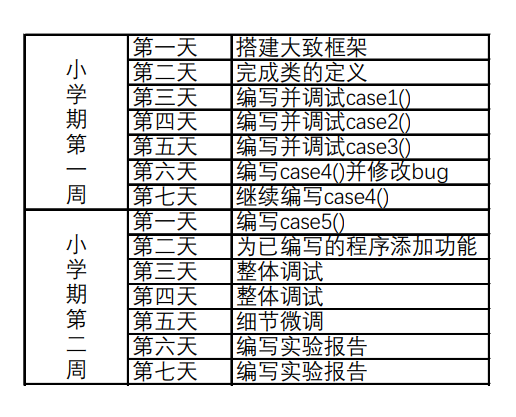
\includegraphics[width = 12cm]{时间规划.png}
	\end{center}
\end{figure}
\vspace*{-2cm}
\section*{评价表}
\addcontentsline{toc}{section}{评价表} 
\vspace*{-0.5cm}
\begin{figure}[h!]
	\begin{center}
		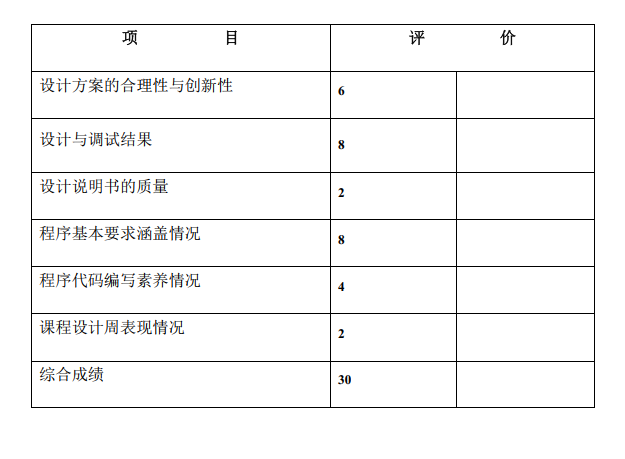
\includegraphics[width = 15cm]{评价表.png}
	\end{center}
\end{figure}


\end{document}\